\documentclass[a4paper,12pt]{article}
\usepackage[utf8]{inputenc}

\usepackage[top=2cm,bottom=2cm,right=1.5cm,left=1.5cm]{geometry}
\usepackage{amsmath,amssymb,enumitem,multicol,graphicx,tikz,framed,tcolorbox,mathtools,comment,subcaption,array,pgfplots}
\usepackage{listings}
\usepackage{xcolor}
\linespread{1.3}
\setlength\parindent{0pt}
%--------------------------
\usepackage{hyperref}
\hypersetup{
	colorlinks=true,
	linkcolor=blue,
	filecolor=magenta,      
	urlcolor=cyan,
}
%New colors defined below
\definecolor{codegreen}{rgb}{0,0.6,0}
\definecolor{codegray}{rgb}{0.5,0.5,0.5}
\definecolor{codepurple}{rgb}{0.58,0,0.82}
\definecolor{backcolour}{rgb}{0.95,0.95,0.92}
\definecolor{backcolour_two}{rgb}{1,1,1}

%Code listing style named "mystyle"
\lstdefinestyle{mystyle}{
  backgroundcolor=\color{backcolour},   commentstyle=\color{codegreen},
  keywordstyle=\color{magenta},
  numberstyle=\tiny\color{codegray},
  stringstyle=\color{codepurple},
  basicstyle=\ttfamily\footnotesize,
  breakatwhitespace=false,         
  breaklines=true,                 
  captionpos=b,                    
  keepspaces=true,                 
  numbers=left,                    
  numbersep=5pt,                  
  showspaces=false,                
  showstringspaces=false,
  showtabs=false,                  
  tabsize=2
}

\lstdefinestyle{mystyle_big}{
	backgroundcolor=\color{backcolour_two},   commentstyle=\color{codegreen},
	keywordstyle=\color{magenta},
	numberstyle=\tiny\color{codegray},
	stringstyle=\color{codepurple},
	basicstyle=\ttfamily\normalsize,
	breakatwhitespace=false,         
	breaklines=true,                 
	captionpos=b,                    
	keepspaces=true,                 
	numbers=left,                    
	numbersep=5pt,                  
	showspaces=false,                
	showstringspaces=false,
	showtabs=false,                  
	tabsize=2
}

%"mystyle" code listing set
\lstset{style=mystyle}

\title{Code Listing}
\date{ }
\begin{document}
	\Large
	\textbf{Level 1 }\\
	\textbf{Iterative Processes Course Notes }
	\normalsize
	\tableofcontents
\newpage
\section{Introduction}


\newpage



\newpage
\section{Dinner Order - Basic Program - Design and Build}
You need to create a program that allows a waiter to enter in the number of main meals ( at \$12.50 each ) , the number of desserts ( at \$6.00 each ) and the number of drinks ( at \$3.55 ) ordered at a table.\\
The program then prints out a summary of the order, a total and then adds on GST (and gives the new total ).\\
(Note: the program should be easy to alter so the price values should be declared as constant variables)


\begin{figure} [!h]
	\centering
	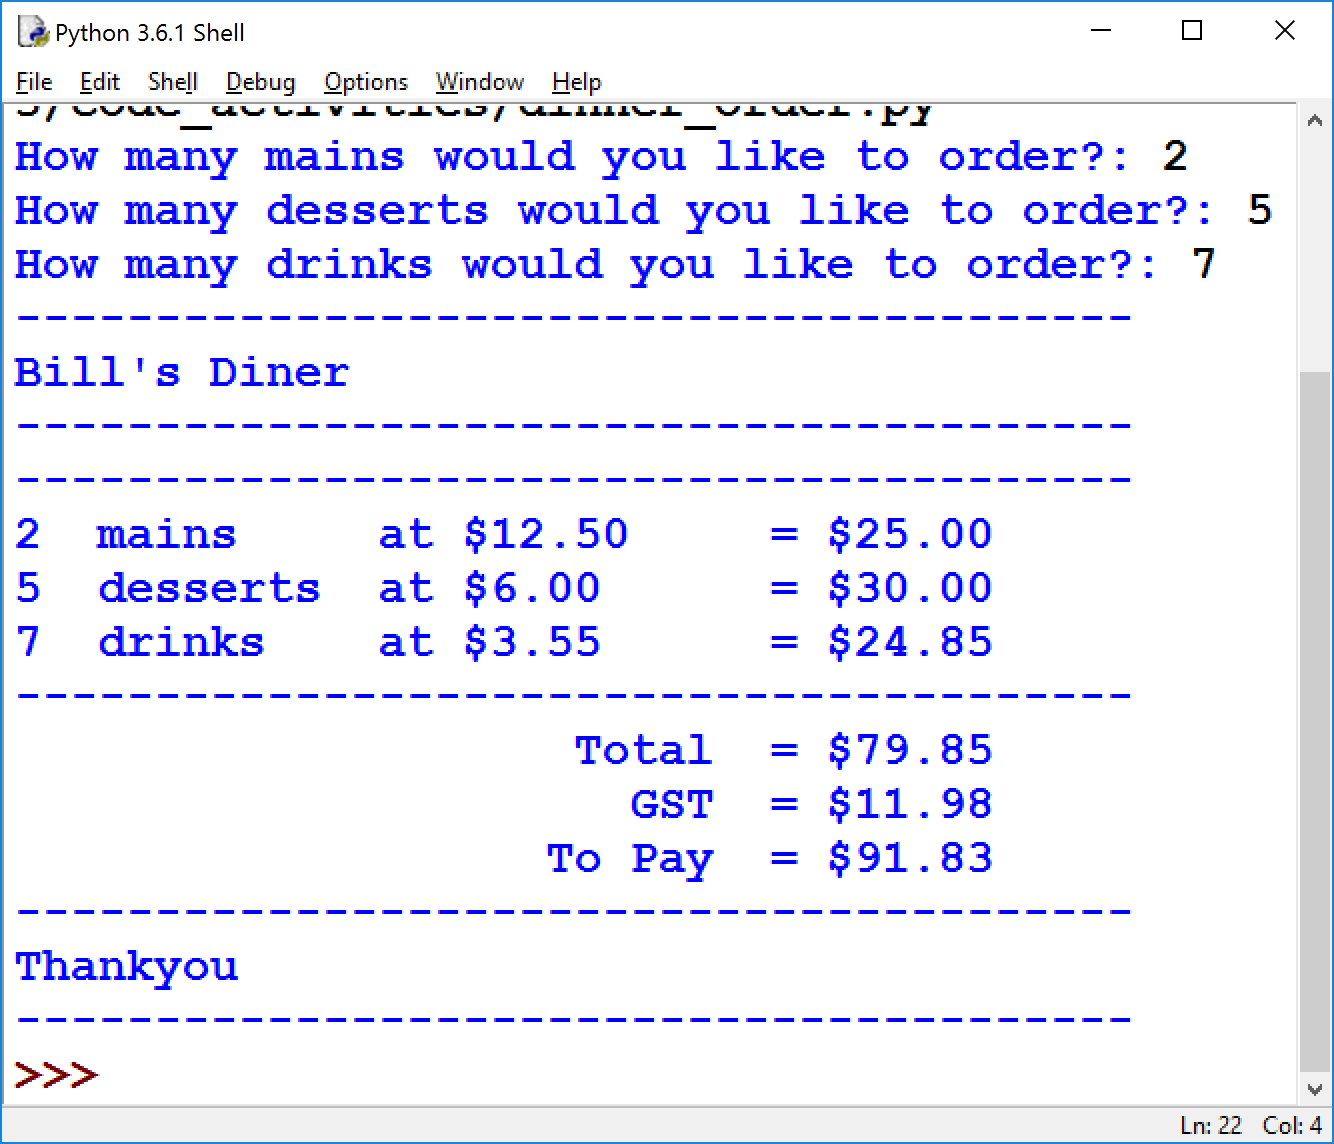
\includegraphics[width=10cm]{screen_shots/diner.png}
	\caption*{An example of Dinner Order program run}
\end{figure}


\subsubsection{Planning}
For the writing and planning:
\begin{itemize}
	\item \textbf{Decomposition}
Please write down your task decomposition.\\
(This is breaking the task down into smaller pieces that will be combined to make the finished program)\\
See examples below.
\item \textbf{Version Log}\\
Your version log should go here.  Annotated screenshots are a good idea at this point
\item \textbf{Component Trialling}\\
Show that you have trialled each component here.  \\
You should also include notes that justify the major decisions you made.
\item \textbf{Assembled Outcome Testing}\\
Please show testing for your assembled outcome below. \\
This should include a test plan followed by screenshot proof
\item \textbf{Usability Testing}\\
Try the program out on someone else and make notes or video etc.
Write a list of things improvements which need to be made based on your usability testing.  Then write down what you changed.
\item \textbf{General Evaluation:}\\
How good is may program? What can I do to improve it?
\end{itemize}


\textbf{Examples of Component Planning}\\
\begin{figure} [!h]
	\centering
	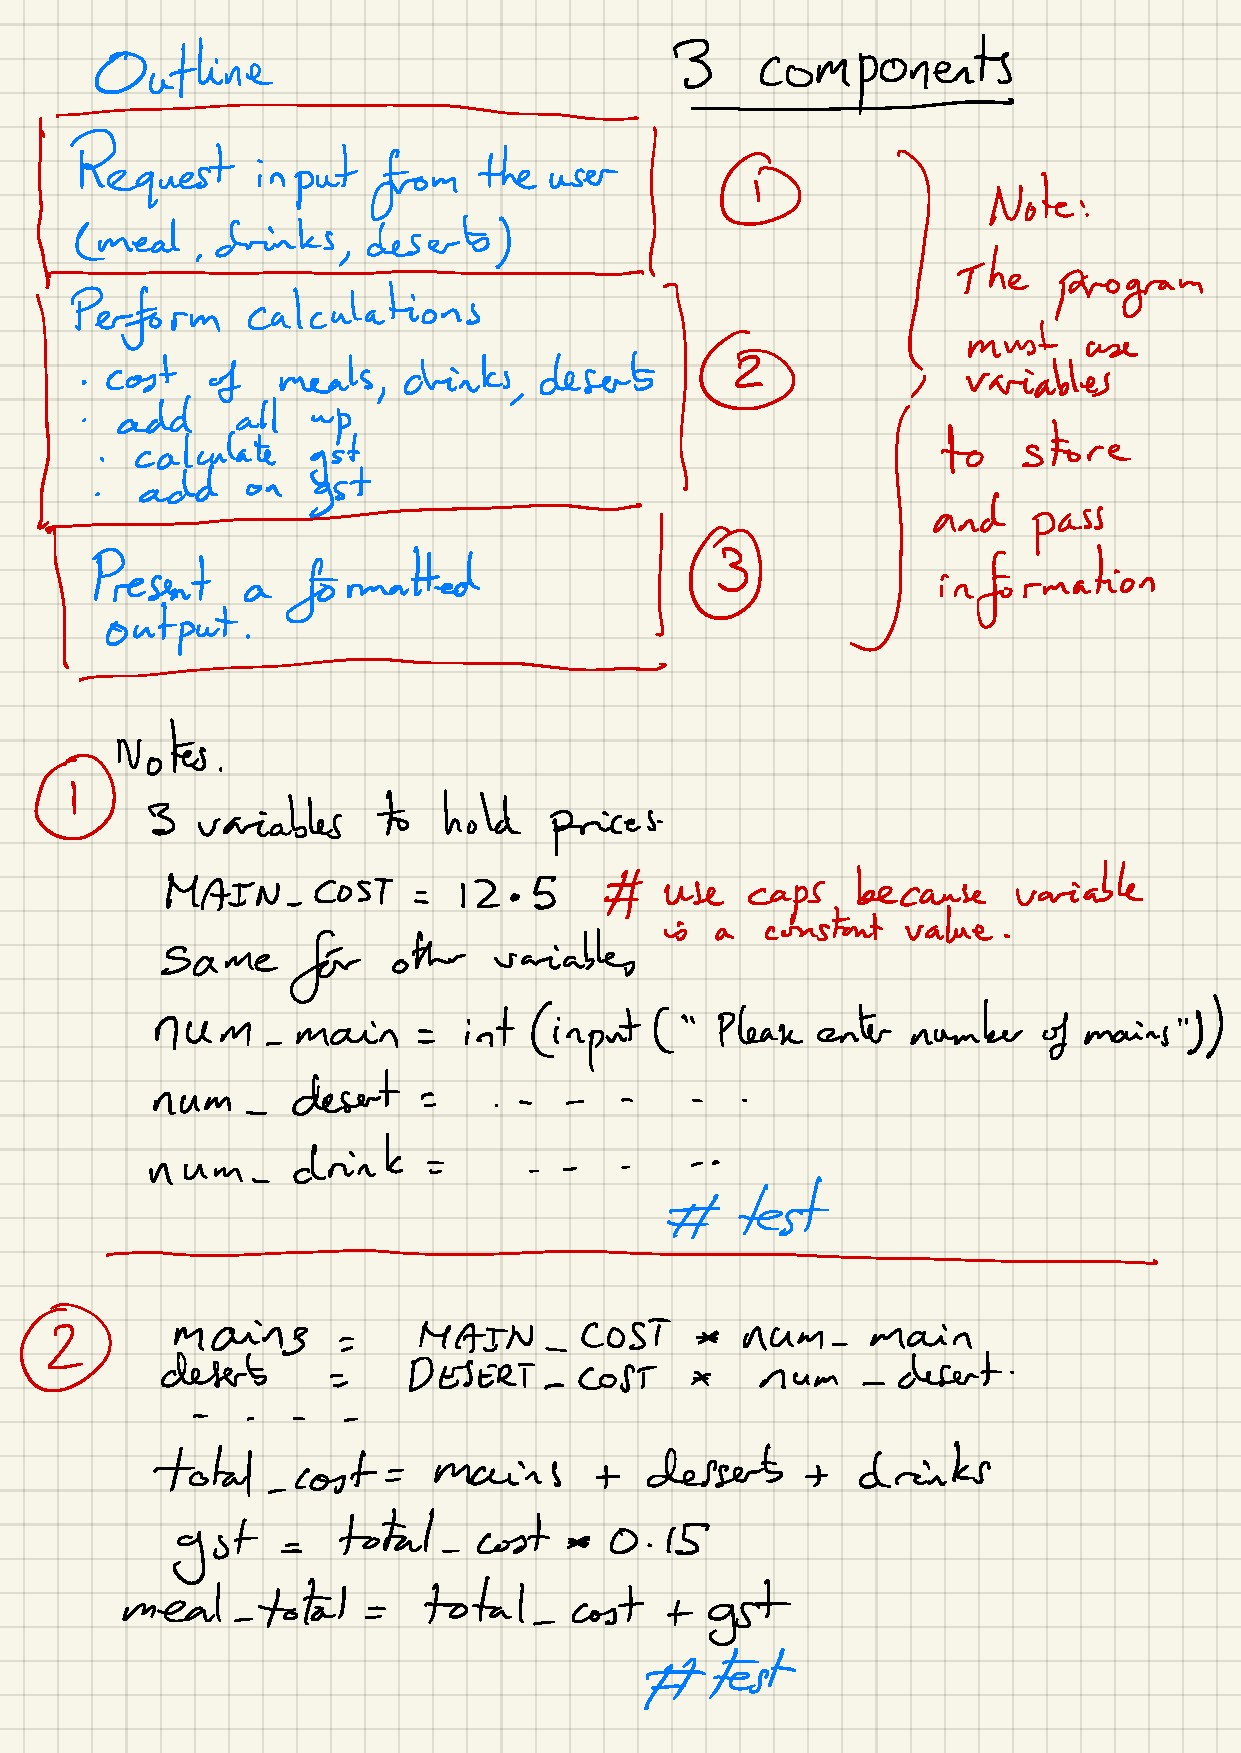
\includegraphics[width=12cm]{iterative_processes/simple_planning_1.pdf}
\end{figure}
\begin{figure} [!h]
	\centering
	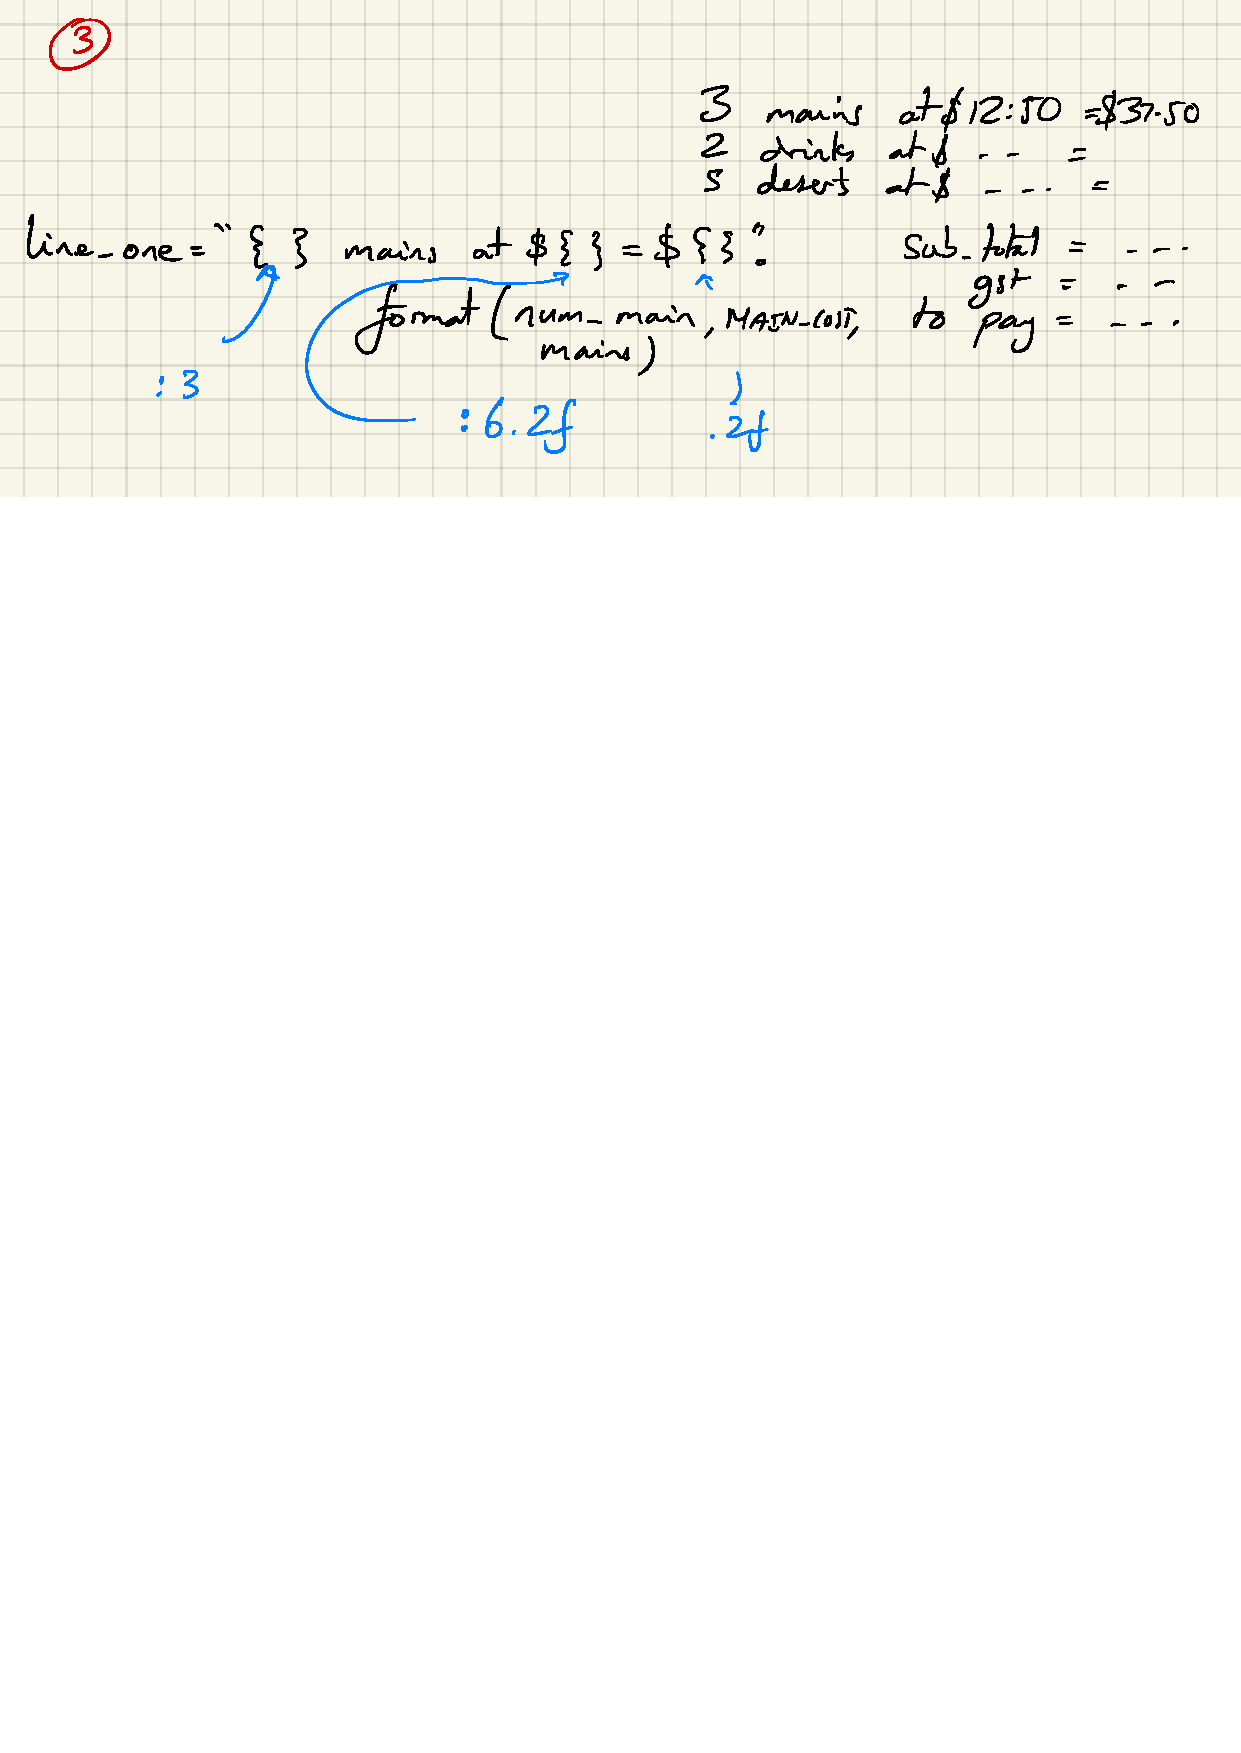
\includegraphics[width=12cm]{iterative_processes/simple_planning_2.pdf}
\end{figure}
\textbf{Basic Idea of Testing}
When testing we consider
\begin{itemize}
	\item Expected inputs (these are inputs we would normally expect the user to input).\\
	Does the porgram give the right outputs with the given expected inputs.
	\item Boundary inputs (are there maximum or minimum value that the user can enter)\\
	What happens at these \underline{boundaries} (and if we go over them)
	\item Unexpected Inputs  (these are character entries that we are not expecting)\\
	These could be just pressing enter or having spaces , using letters instead of numbers or characters like * , \&, etc.\\
	These could occur if the user makes a mistake or misunderstands what is expected.
\end{itemize}
Testing should have some kind of plan and documentation of the results.\\

\begin{figure} [!h]
	\centering
	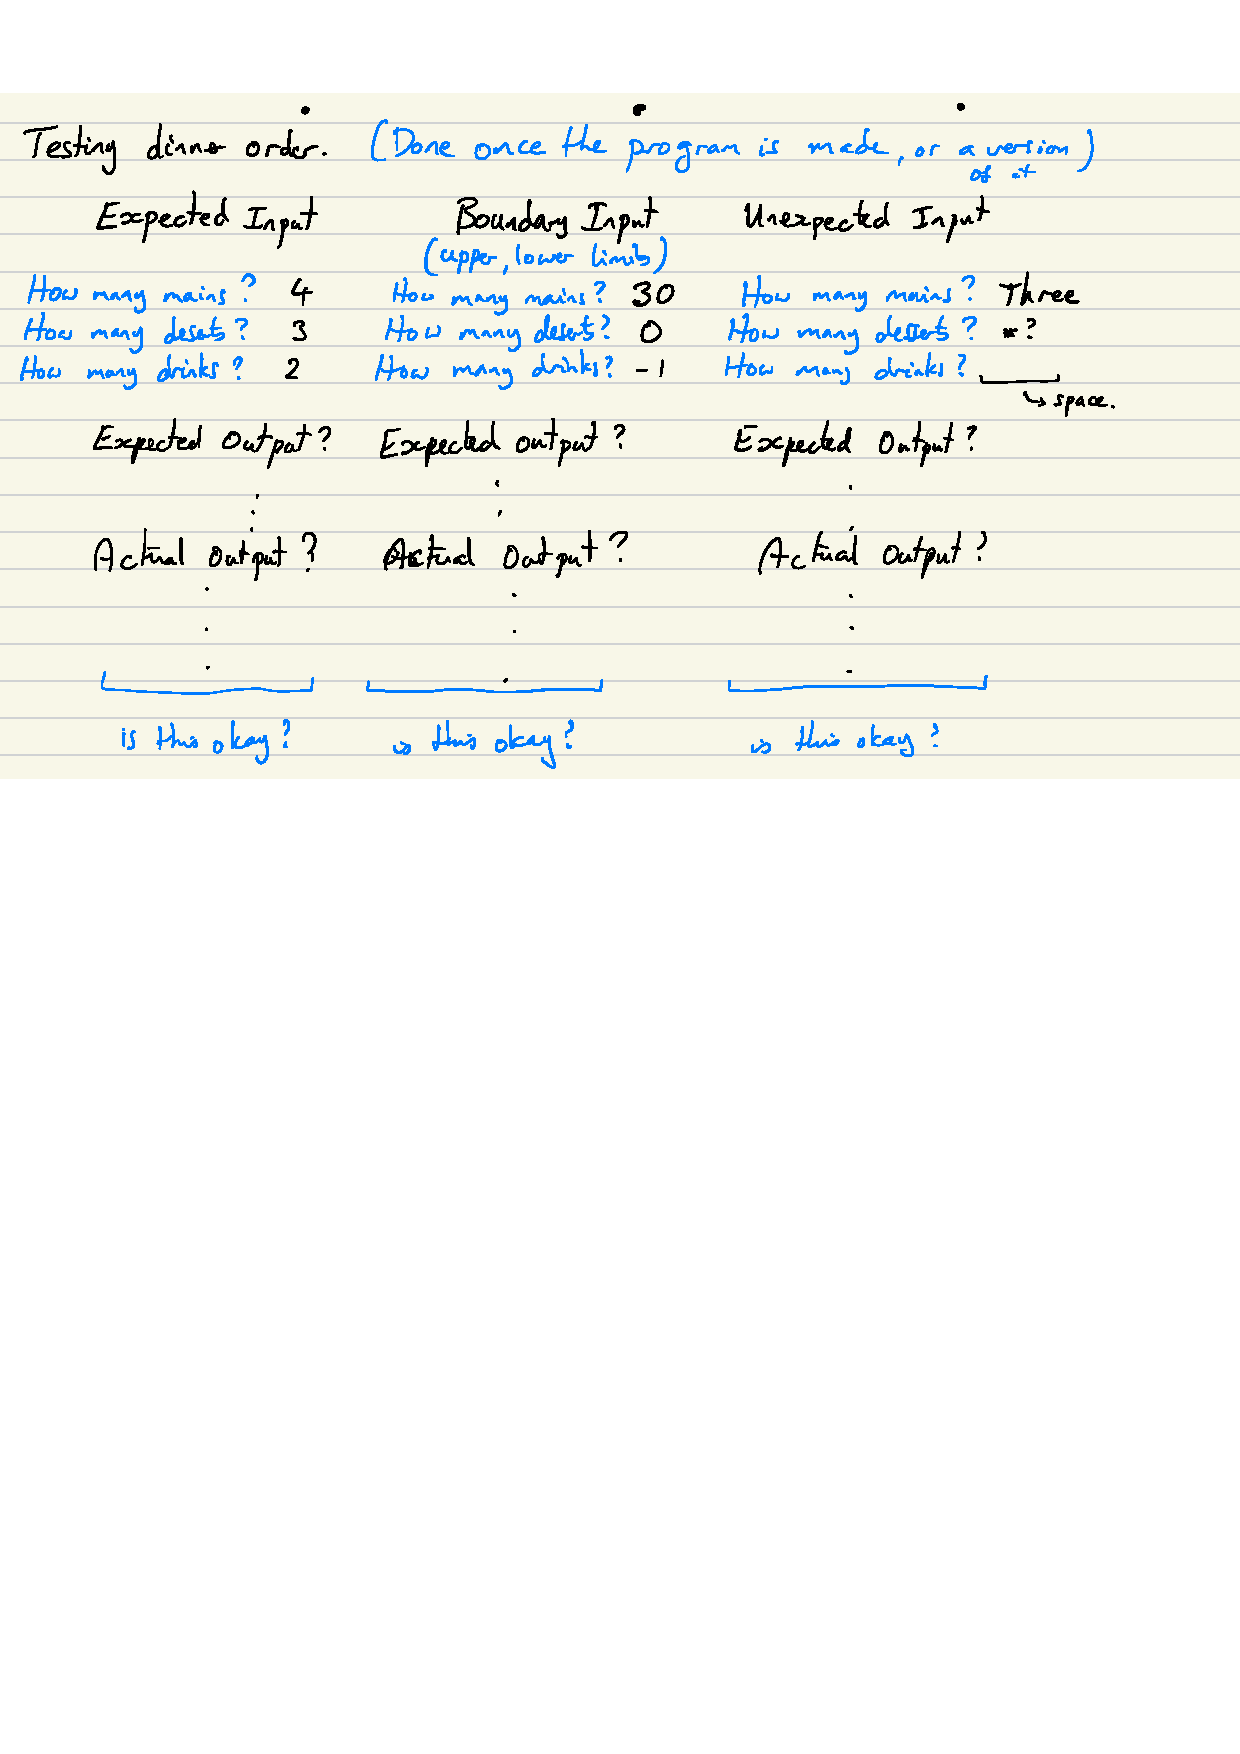
\includegraphics[width=16cm]{iterative_processes/Testing.pdf}
\end{figure}

\begin{figure} [!h]
	\centering
	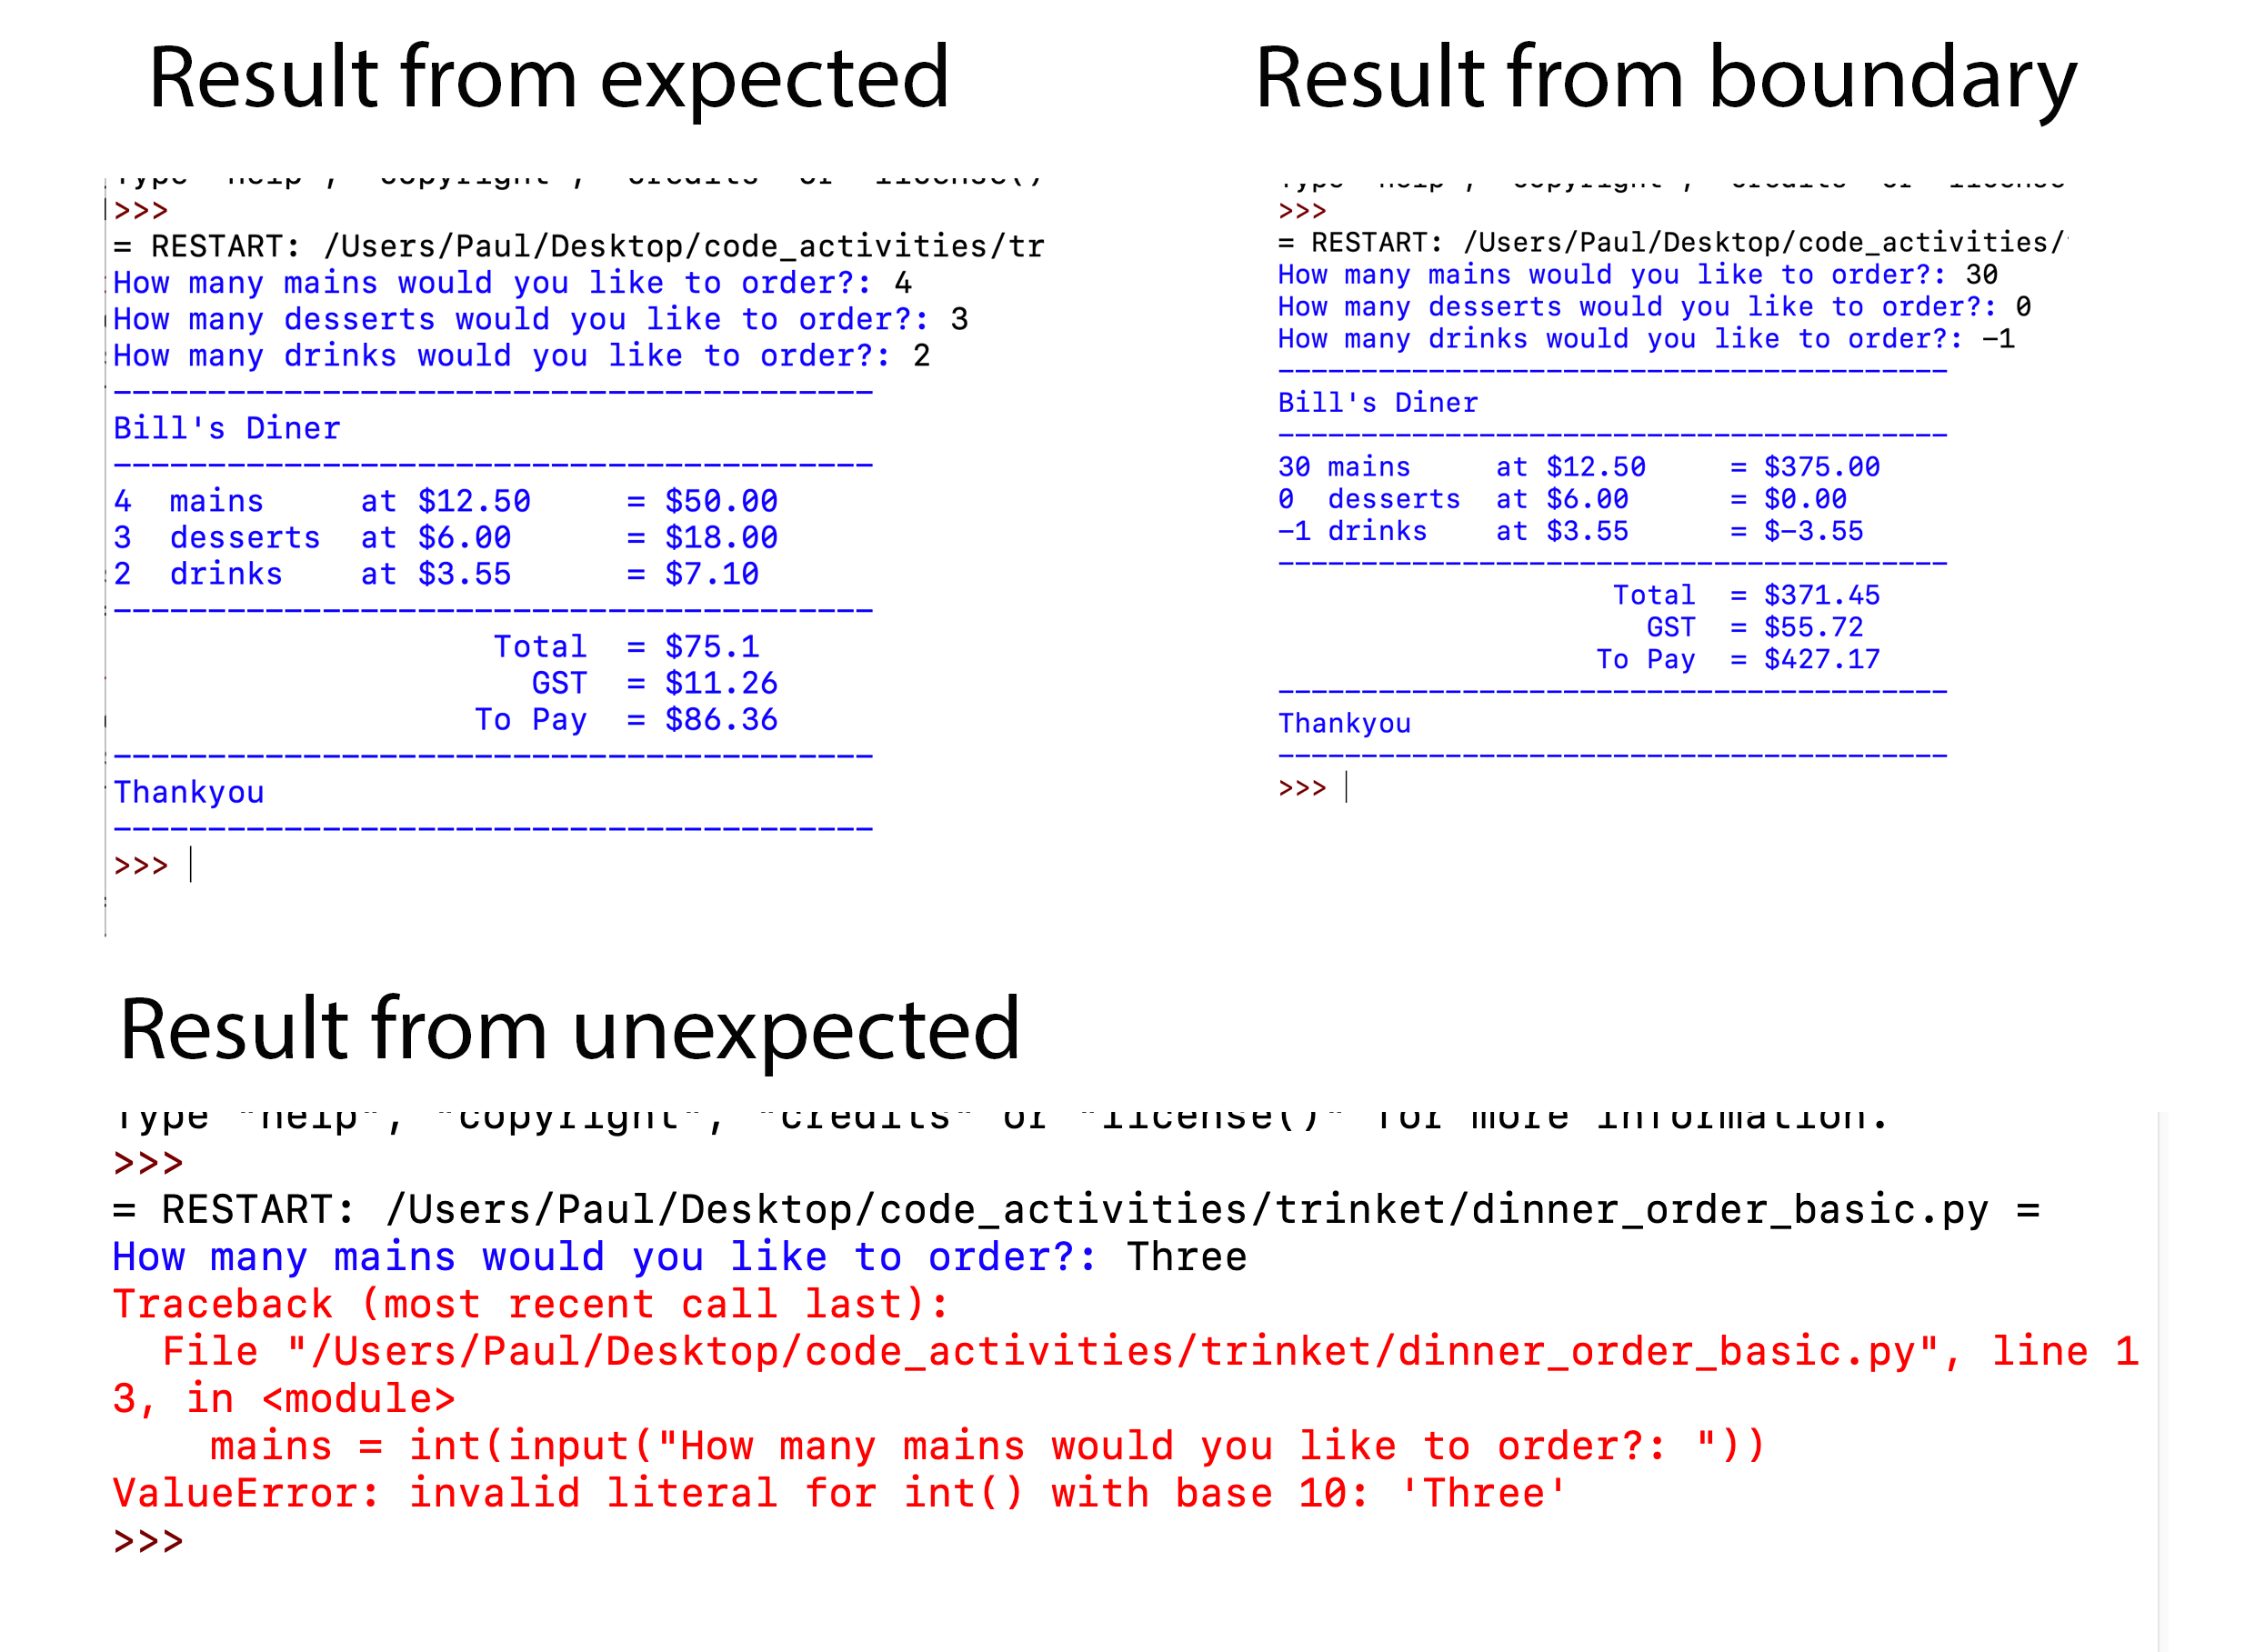
\includegraphics[width=16cm]{iterative_processes/Testing.png}
\end{figure}
\newpage
\textbf{Evaluation}
\begin{itemize}
	\item What works 
\begin{itemize}
	\item Works properly on expected inputs
	\item Presentation of reciept clearly laid out on console.
\end{itemize}
	\item What could be improved
\begin{itemize}
	\item Should have an upper limit on how many meals can be entered
	\item Should not allow entries below zero
	\item Unexpected inputs cause a program crash
	\item At the moment the program only runs once (so need a way to enter a new order)
\end{itemize}
\end{itemize}
\newpage

\begin{figure} [!h]
	\centering
	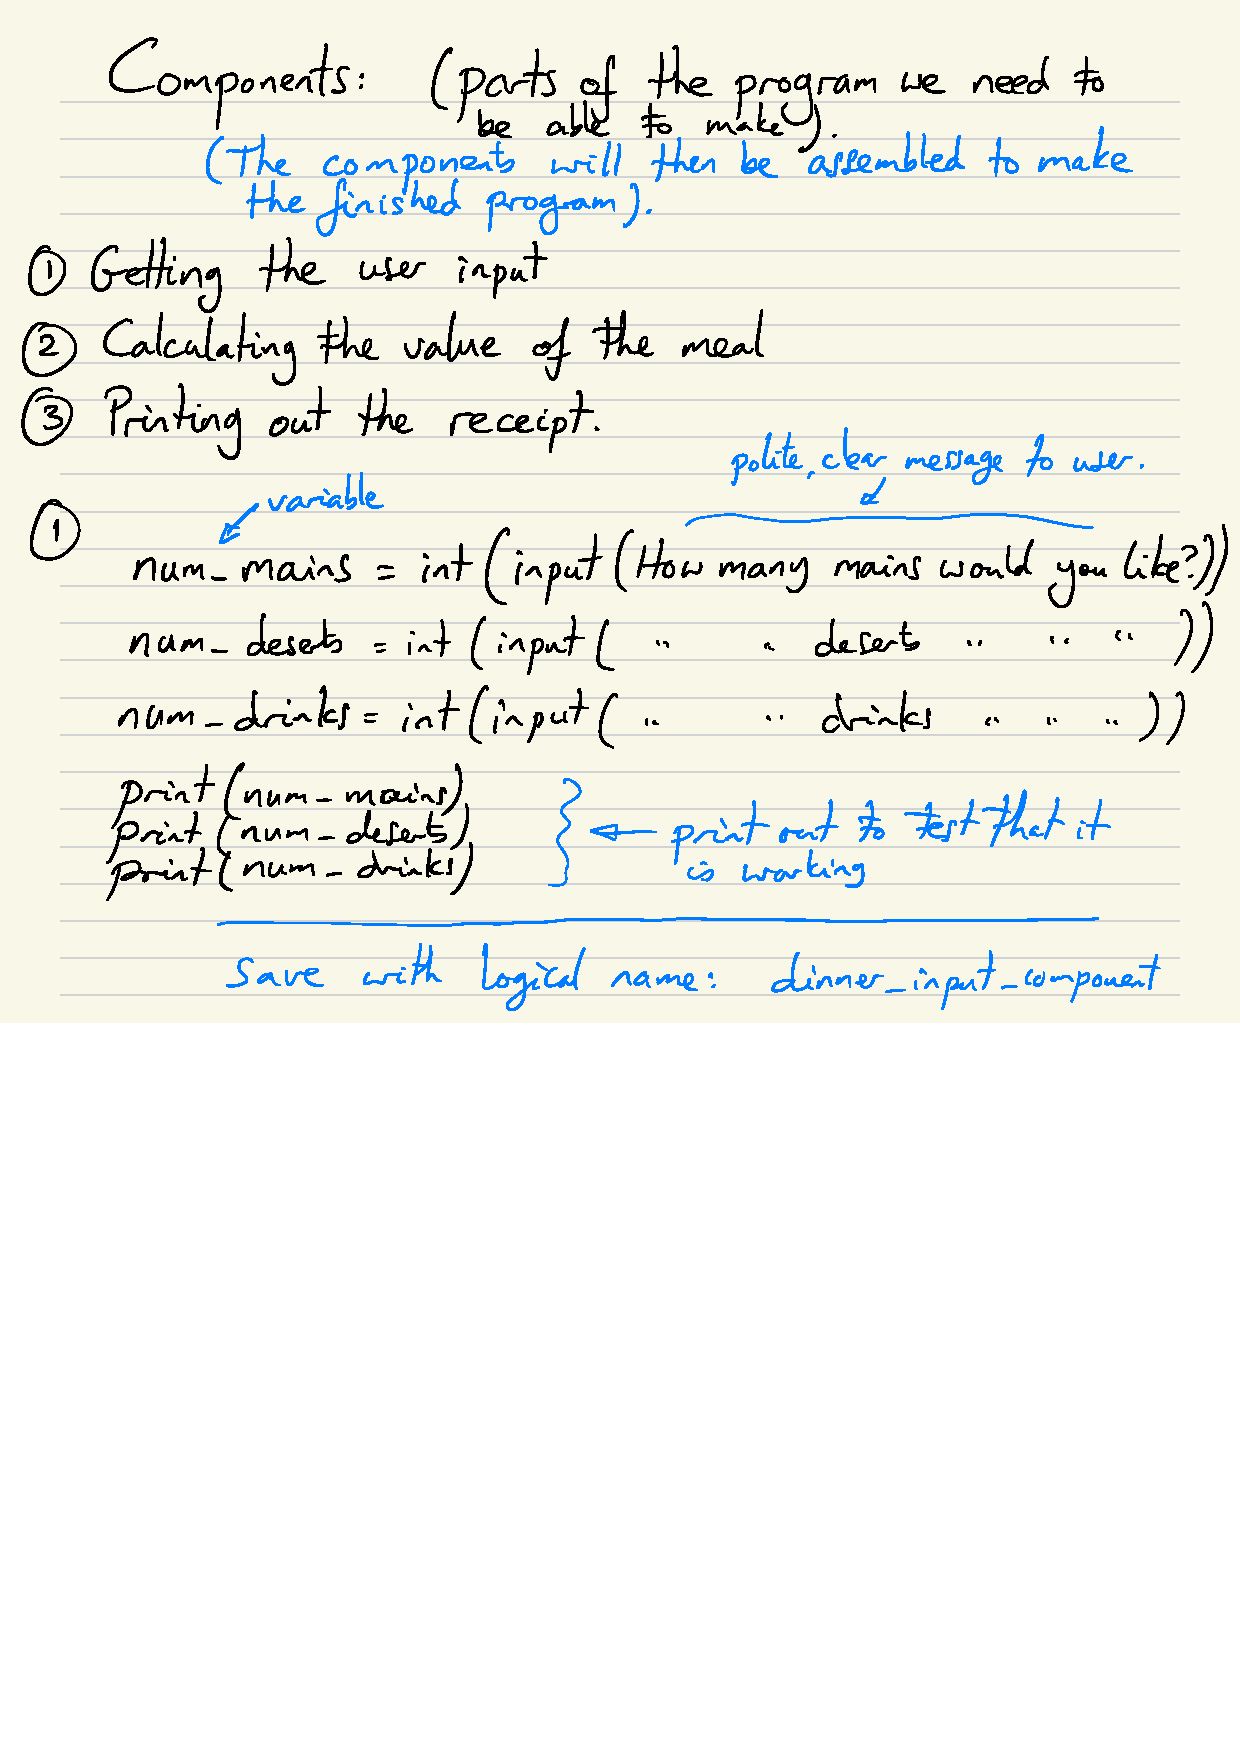
\includegraphics[width=8cm]{iterative_processes/Components_detailed_p1.pdf}
\end{figure}
\begin{figure} [!h]
	\centering
	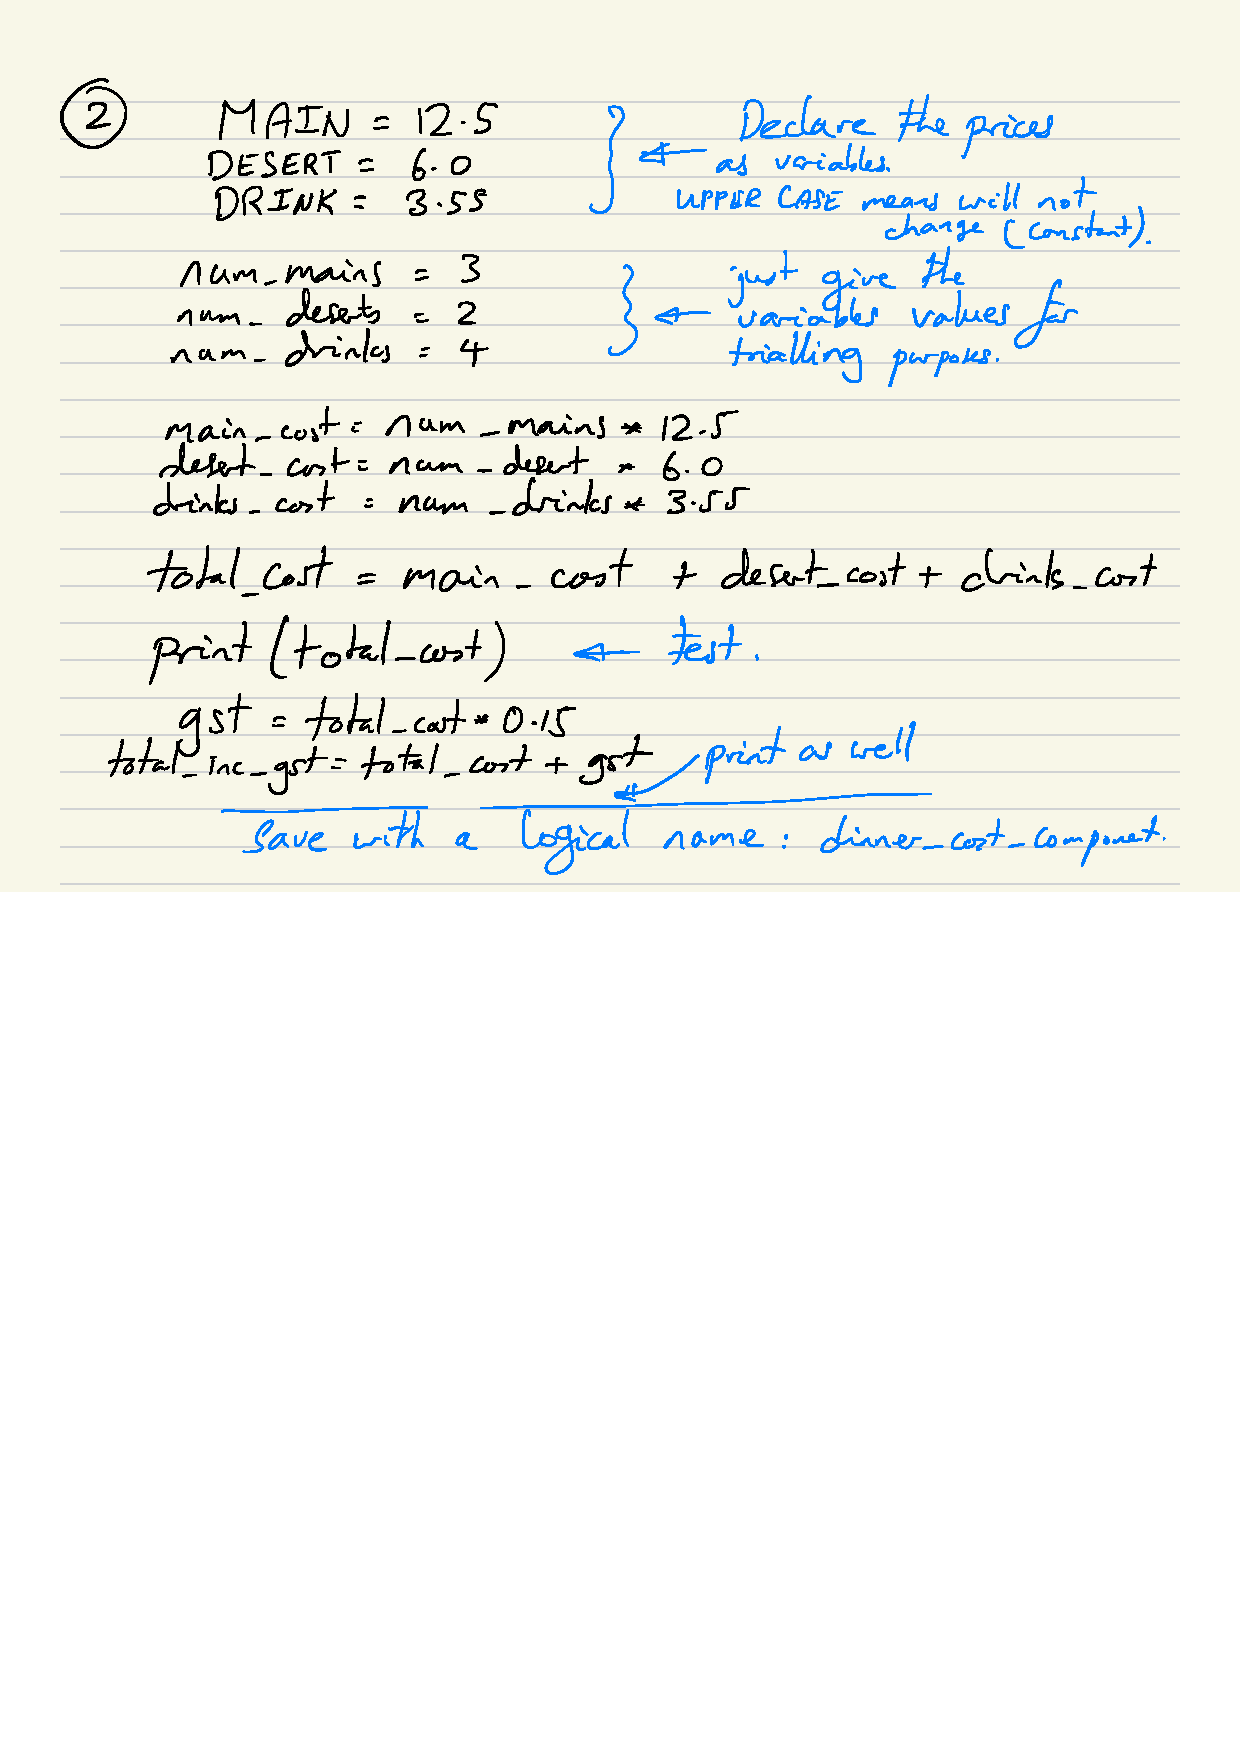
\includegraphics[width=8cm]{iterative_processes/Components_detailed_p2.pdf}
\end{figure}


\begin{figure} [!h]
	\centering
	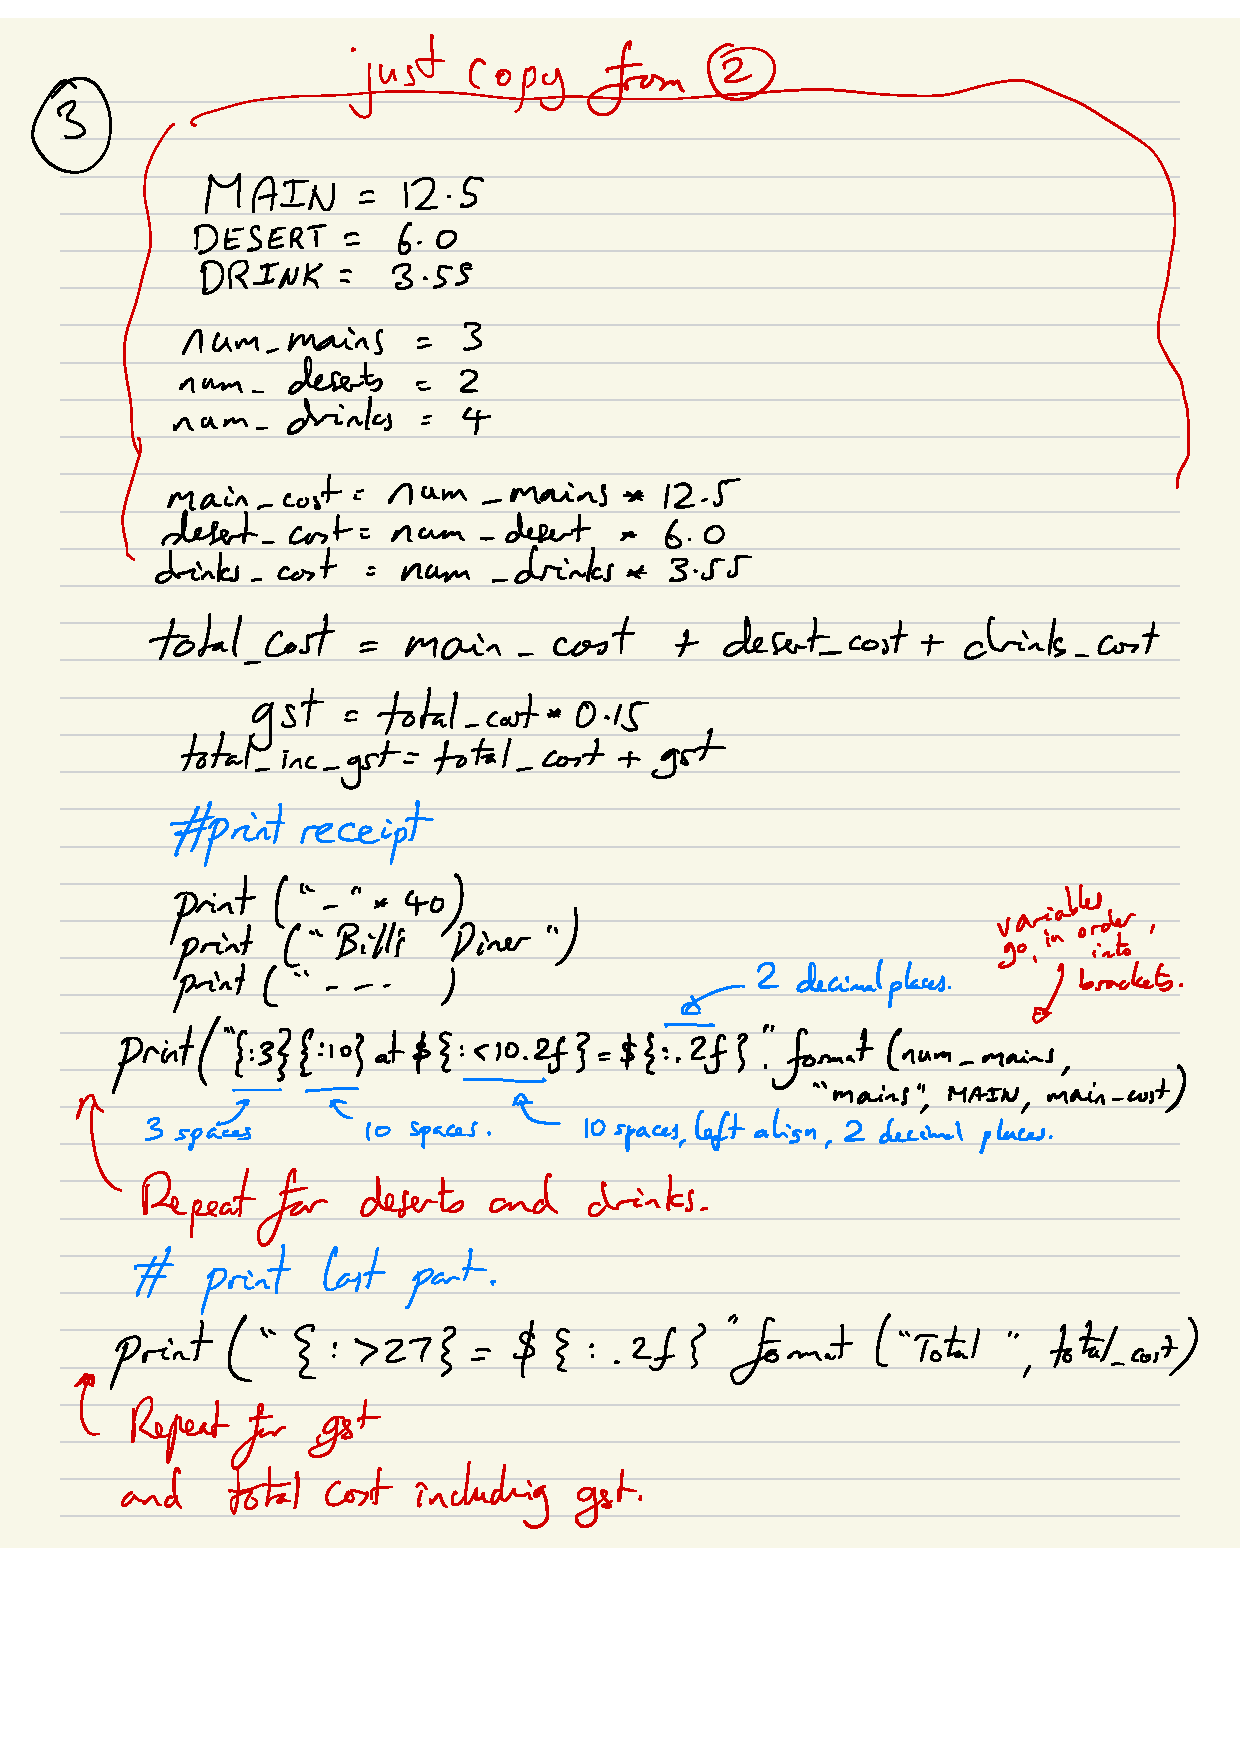
\includegraphics[width=8cm]{iterative_processes/Components_detailed_p3.pdf}
\end{figure}

\newpage


\lstinputlisting[language=Python, caption = Dinner Order Program]{trinket/dinner_order_basic.py}

\newpage
\subsection{Strawberry picking}

A strawberry farm lets families come and pick strawberries. \\
They can fill boxes, buckets or punnets (any combination).\\
\begin{itemize}
	\item They charge a rate of 5 \$/kg. 
	\item Full of strawberries, a punnet weighs 250 g, a box weighs 1.5 kg and a bucket weighs 7 kg.
\end{itemize}
Design a program that calculates the amount to be charged given a certain number of boxes, punnets and buckets have been picked.

\begin{figure} [!h]
	\centering
	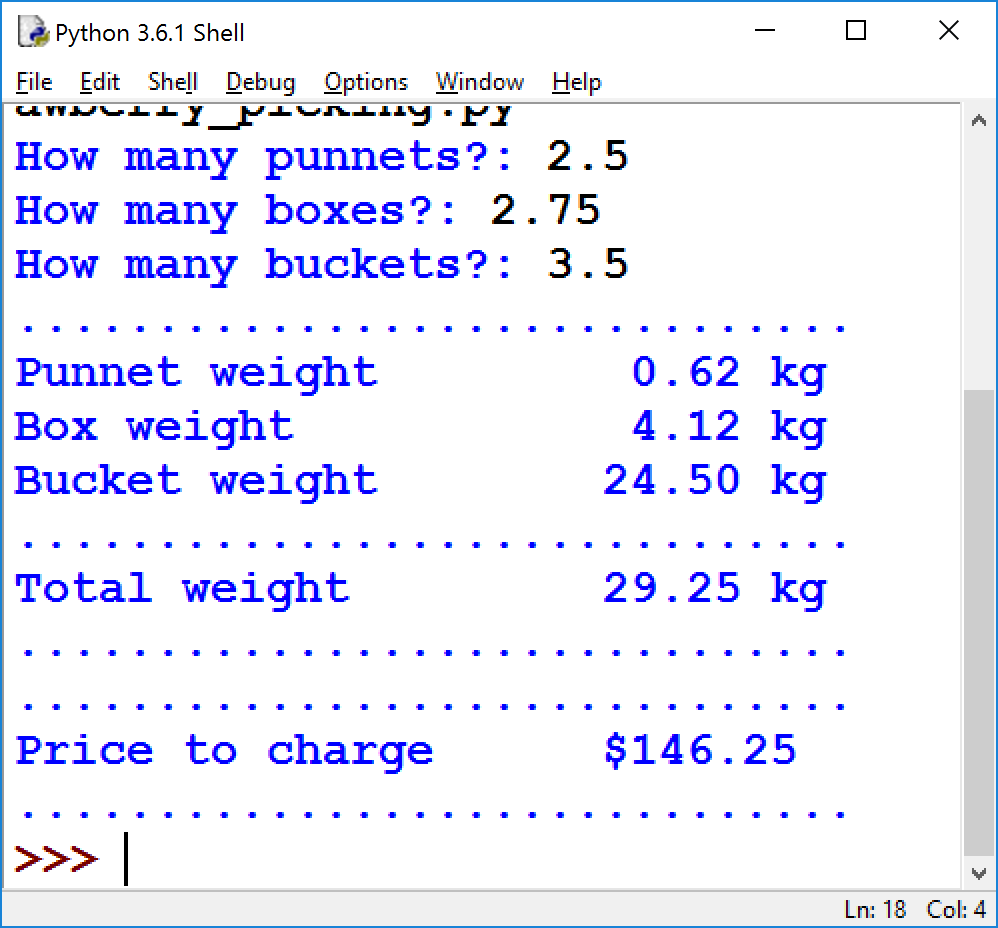
\includegraphics[width=10cm]{screen_shots/strawberries.png}
	\caption*{An example of Strawberries program run}
\end{figure}
\newpage
\lstinputlisting[language=Python, caption=Python example
]{strawberry_picking.py}

\newpage
\section{Conditions - Activities}

\begin{enumerate}
	\item Consider a program that asks for a user’s age and then:
\begin{itemize}
	\item if their age 12 or less, tells them that they should be at primary school,
	\item if there age is more than 12 but less than 18, they need to go to secondary school
	\item if they are 18 years old, it tells them that they have become an adult
	\item and if they are older than 18 tells them that they must have left school.
\end{itemize}
\item 	To go to university a person needs to be:
\begin{itemize}
	\item over the age of 20
	\item \textbf{or} be 16 or older and have level 3 NCEA 
	\item \textbf{and} (for both conditions) the person need to be competent with English.
\end{itemize} 
Create a program that given the following variables:\\
age= 25\\
ncea = False\\
english = True\\
Will give a correct response about whether a person can go to university or not.\\
Test with other values.
\end{enumerate}

\newpage

\section{Guess greater , less or equal.}

Write a program that :\\
Generates a random number between two integers.
\begin{itemize}
	\item It calculates the middle value of the two integers.
	\item It then asks the user to choose whether the random  number is Less than the middle number or More than or Equal to the middle number.
	\item It then gives feedback, saying whether they have won or lost
\end{itemize}

\begin{figure} [!h]
	\centering
	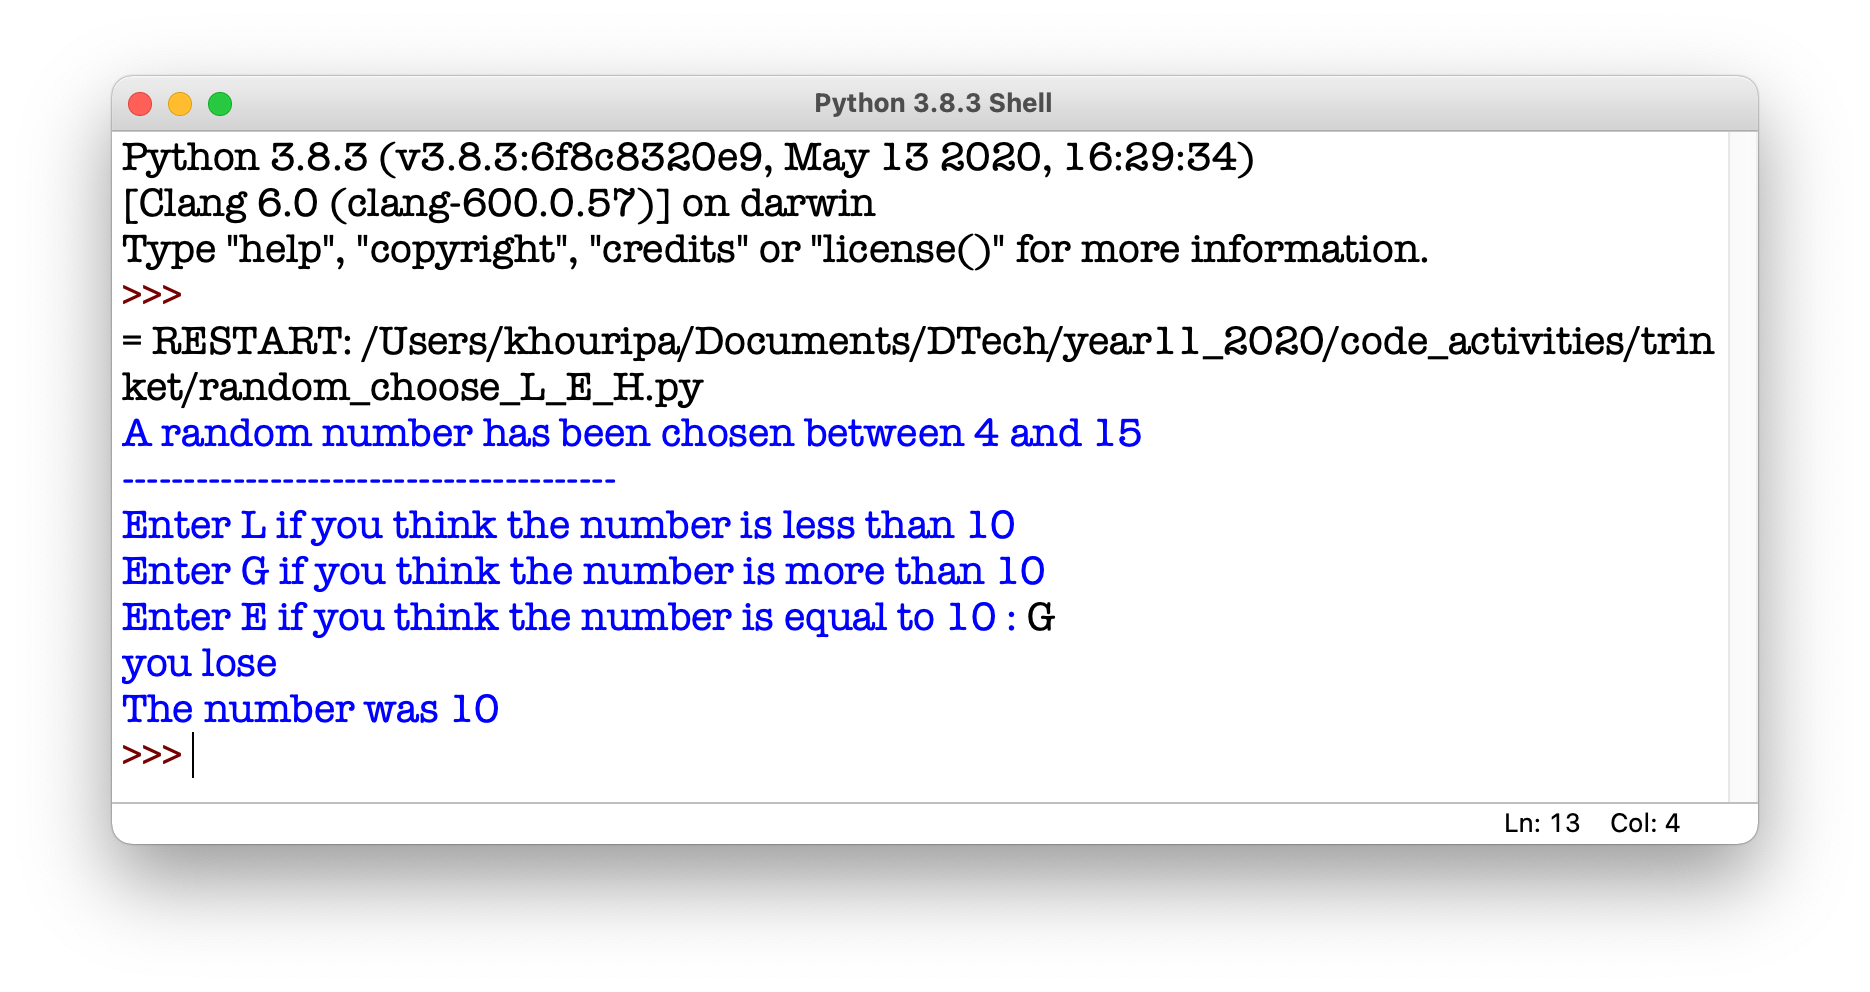
\includegraphics[width=13cm]{screen_shots/random_choose_L_E_H.png}
	\caption*{An example of greater , less , equal  program run}
\end{figure}

For this program:
\begin{itemize}
	\item A pseudo code plan.
	\item Basic test grid.
\end{itemize}
\newpage

\begin{figure} [!h]
	\centering
	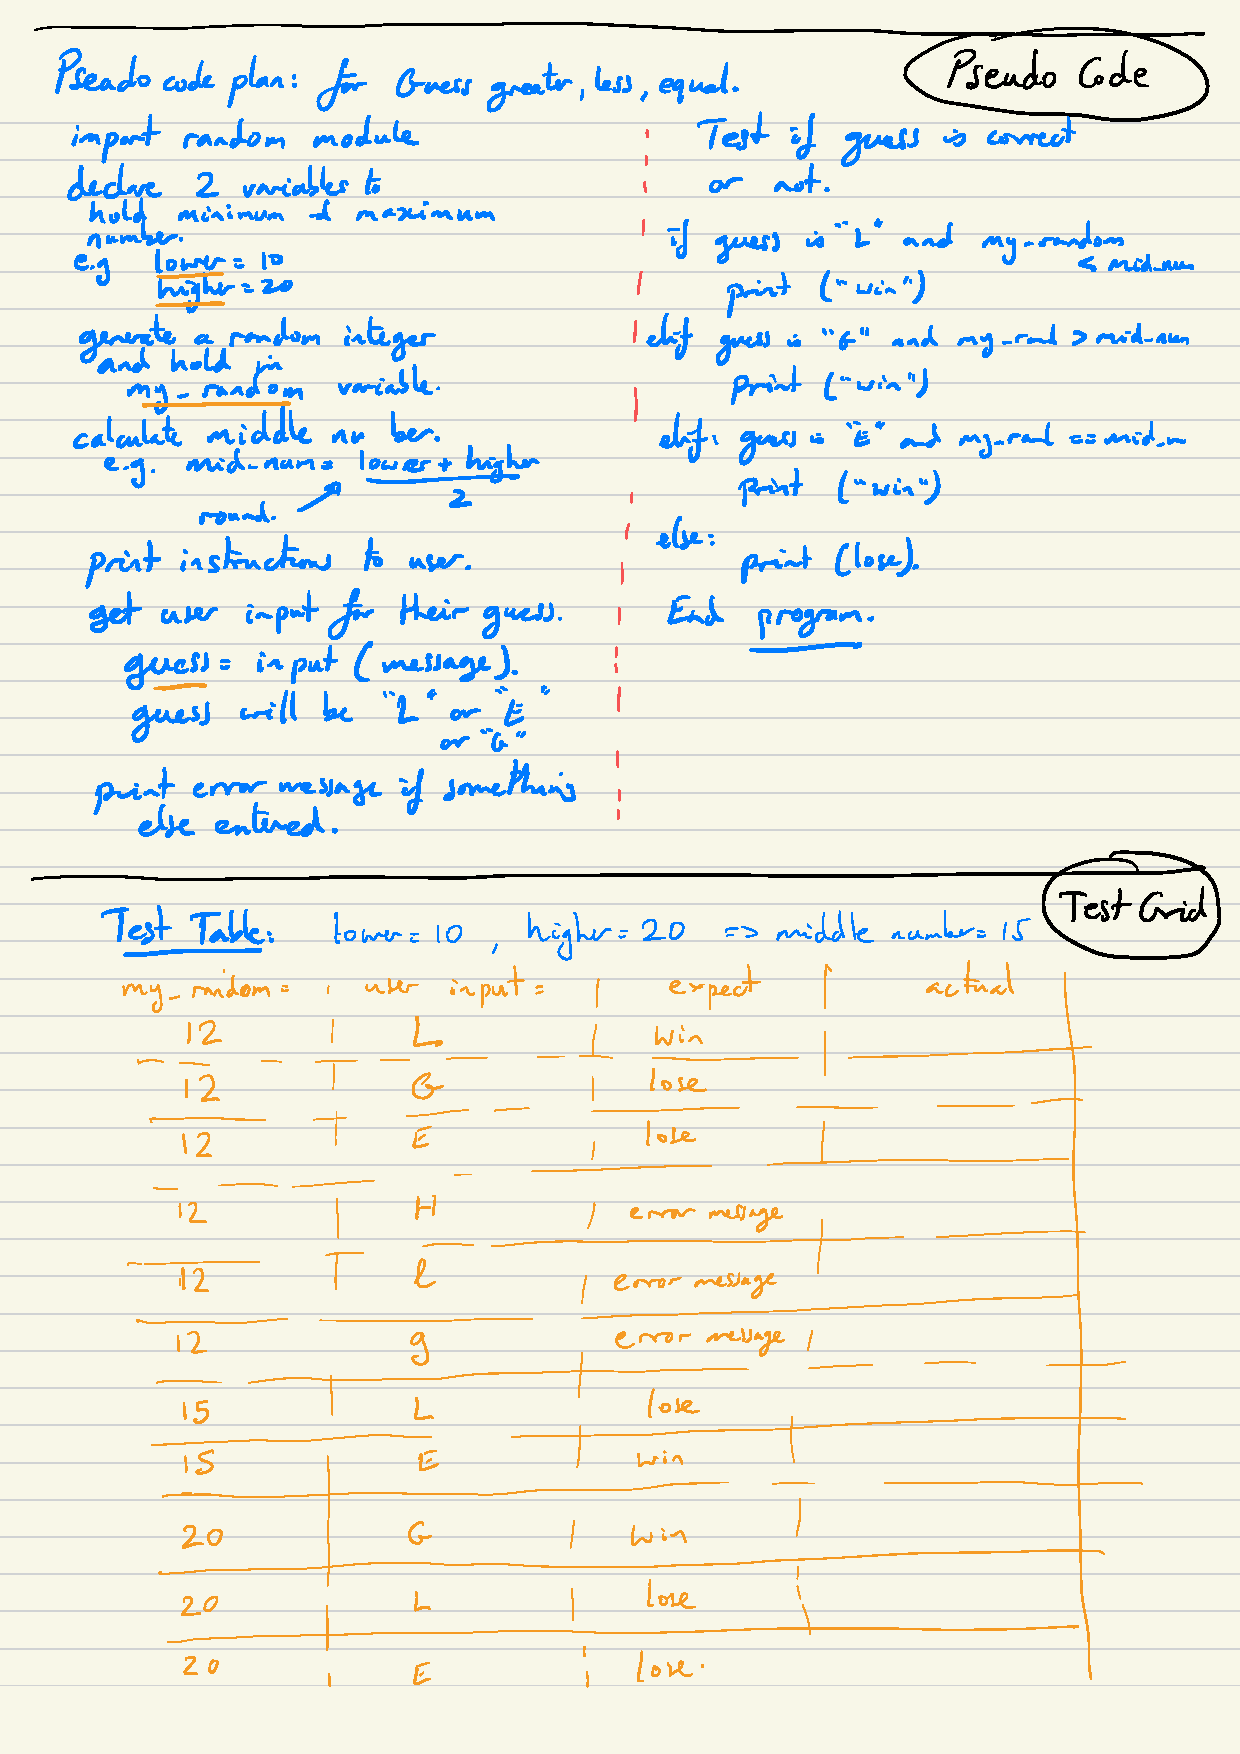
\includegraphics[width=17cm]{iterative_processes/Greater_Less_Equal_planning.pdf}
	\caption*{Psuedo code and test grid}
\end{figure}
\newpage

%\lstset{style=mystyle_big}
\lstinputlisting[language=Python, caption=Python example]{trinket/random_choose_L_E_H.py}
%\lstset{style=mystyle}
\newpage

\section{Loop Activities - improving previously made programs}
Take the Dinner Order and the Guess greater less or equal programs  and make a new version so that they can run more than once.\\
See example: \url{https://sites.google.com/marsden.school.nz/yr11digitaltech2020/computer-program/loops?#h.p_XCtf-2lKZ-CK}\\\\
There is considerable scope now for extension:
Consider:
\begin{itemize}
\item Dinner order prints out total cost of all orders when the program finishes (and/or total mains, deserts, drinks ordered)
\item Guess greater less or equal prints out total score of wins at the end of the program
\item Guess greater less or equal allows the user to bet each time and feeds back on winnings/losses
\end{itemize}

\begin{figure} [!h]
	\centering
	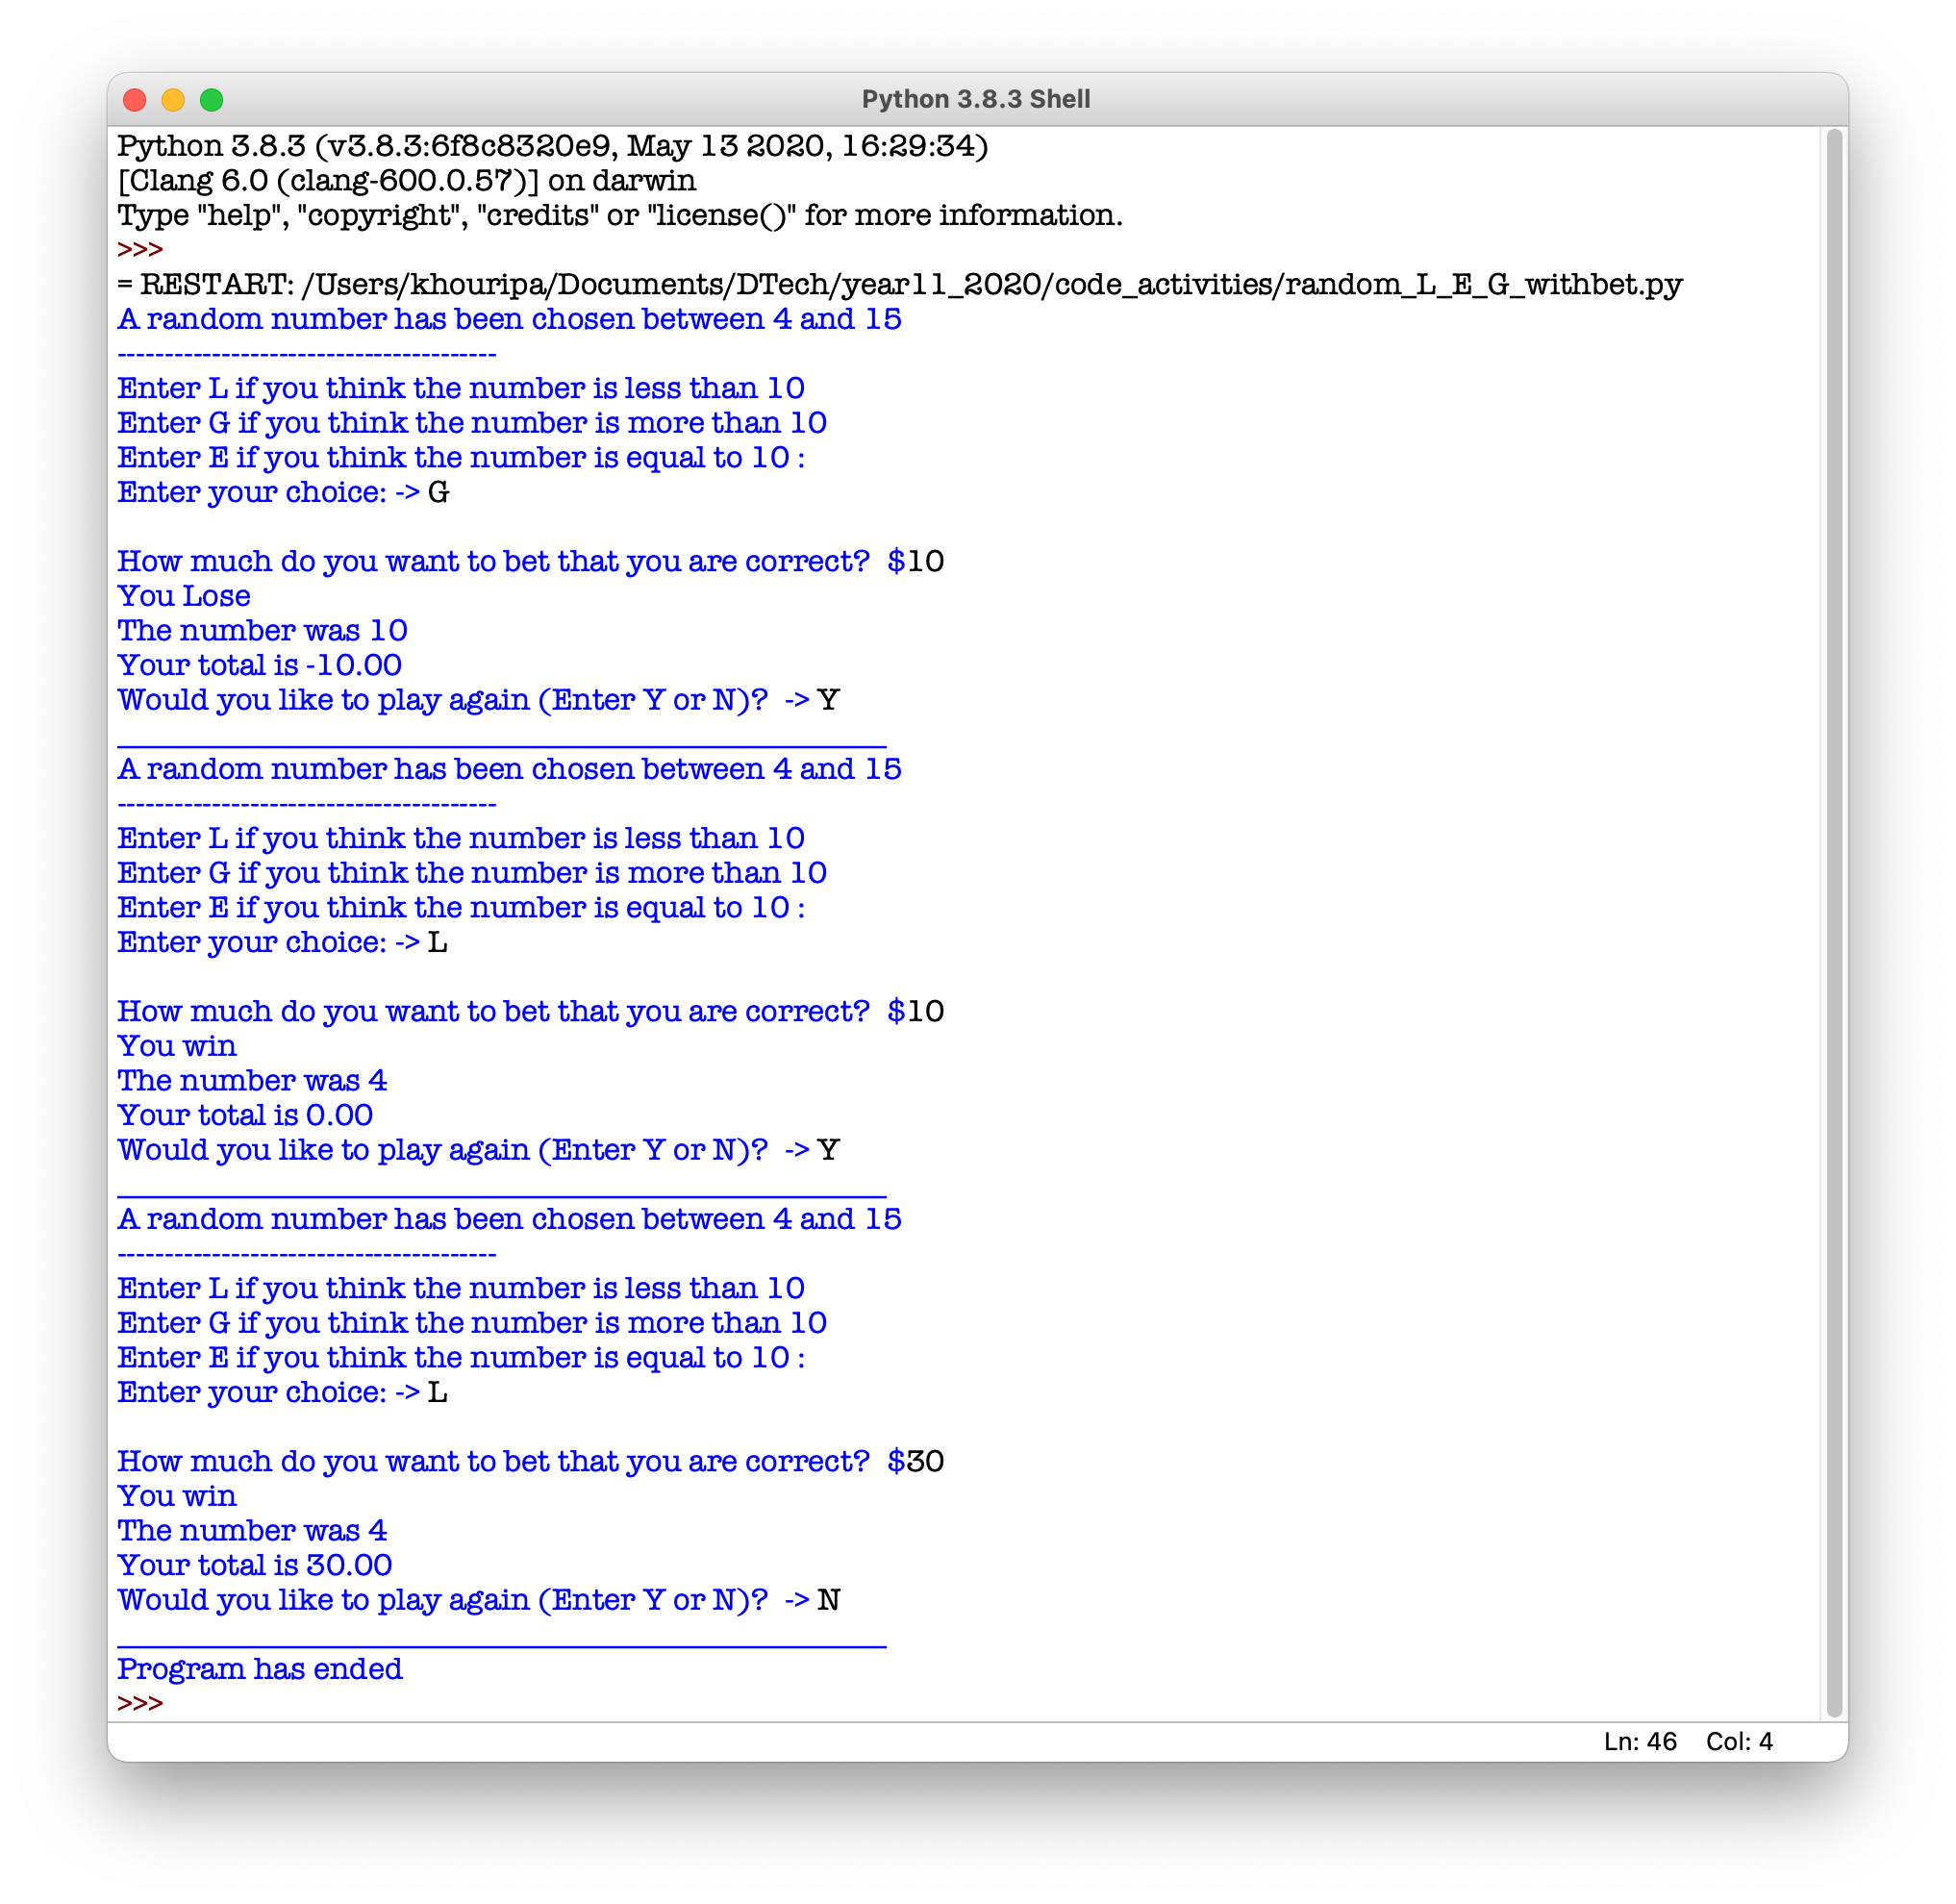
\includegraphics[width=15cm]{iterative_processes/random_L_E_G_withbet.png}
	\caption*{Greater less equal, with loop and betting}
\end{figure}
\newpage
\begin{figure} [!h]
	\centering
	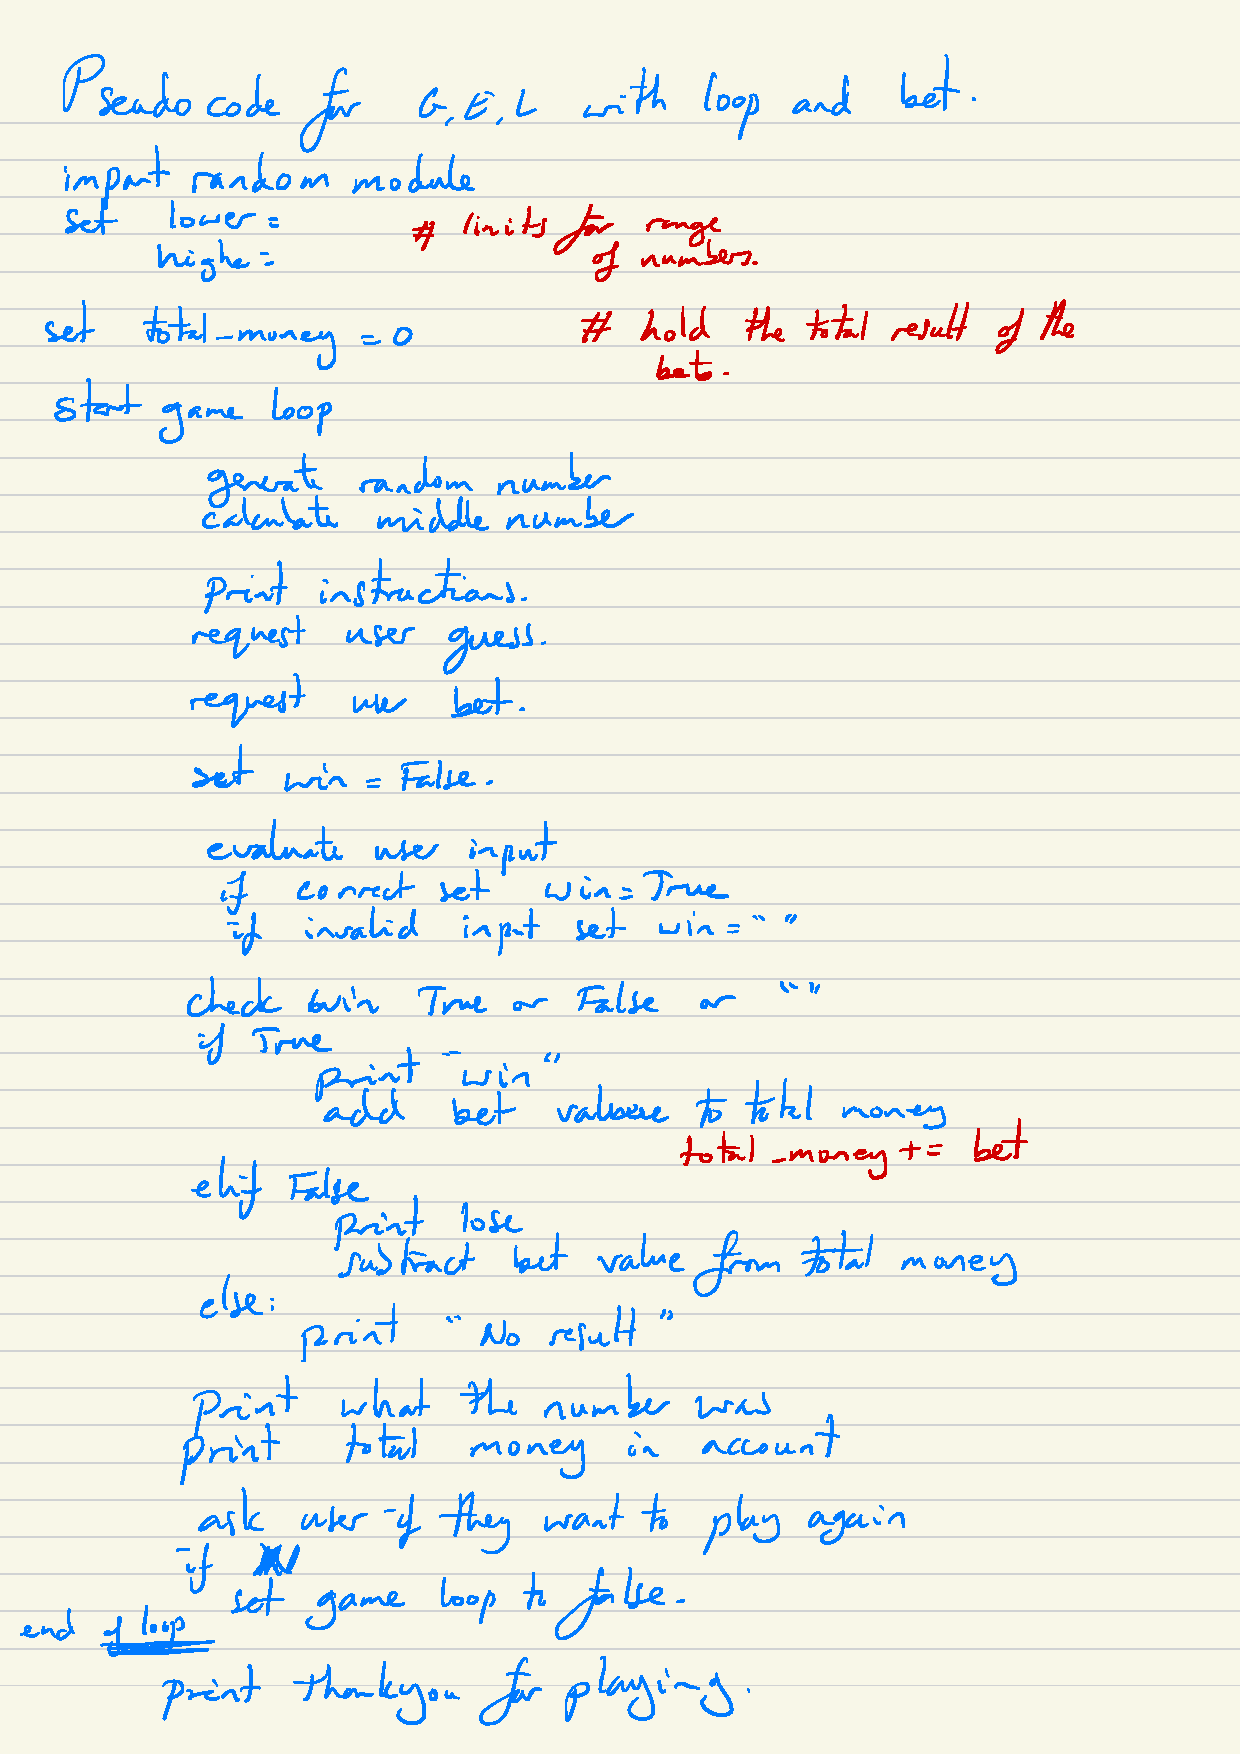
\includegraphics[width=17cm]{iterative_processes/random_L_E_G_withbet.pdf}
	\caption*{Psuedo code: Greater less equal, with loop and betting}
\end{figure}
\newpage
\subsection{Higher Lower Game}
\subsubsection{Program}

\textbf{Scenario:}\\
You have a younger family member who loves the ‘higher / lower’ game so you decide to make a game that they can play whenever they want.\\
\hrule\vspace{0.5cm}
\textbf{Your game should:}
\begin{itemize}
	\item Ask for the user’s name (and address them by their name)
	\item Generate a ‘secret’ number between 1 and 100 and then ask the user to guess the number.
	\item Tell the user if their guess is ‘too high’ or ‘too low’.
	\item If the user correctly guesses the number, the game should congratulate them.
\end{itemize}
If they don’t guess the number in 10 goes, they should be told that they have lost the game and the mystery number should be revealed.\\
\hrule\vspace{0.5cm}
\textbf{Developing the game:}\\
At the end of each game, the user should be asked if they would like to play again

For the ones below, the problems will need to be worked out in a separate small program, before they are implemented in the next version:
\begin{itemize}
	\item Allow the user to choose the lowest and highest number that will be used as the secret number
	\item 	this should be validated, so it is probably a good idea that you have a validation function,
	\item to develop this properly you should be able to validate it so the lower number is less than the high number.
	\item Ideally the game should be set up so that users can’t guess the same *wrong* number twice.
	\item This will require collecting a list of the guessed numbers.
\end{itemize}
\hrule\vspace{0.5cm}
\textbf{Variations (recommended)}:
Please consider adding in the following features.  You should develop (and test) these as part of the problem decomposition.
\begin{itemize}
	\item Allow the user to choose the lowest and highest number that will be used as the secret number
	\item Either allow the user to choose the number of guesses or set a sensible limit based on the difference between the highest and lowest number.
	\item Ask the user how many rounds they would like to play in a given game.  Choose a sensible maximum for this and justify your decision
	\item Keep track of the number of rounds played and the user’s scores
	\item At the end of the given number of rounds, tell the user what their best, worst and average scores were.  Ask them if they wish to play again.
\end{itemize}
\hrule\vspace{0.5cm}


\subsubsection{Planning}
\textbf{Task:}\\
As well as a working program , you need to provide evidence showing how the problem has been decomposed,  how the components have been developed and trialled, and of how they have been assembled and tested to create a final, working outcome.\\

Decompose the problem (write down the decomposition on the template supplied)\\
For each part of the problem, write (and test) each piece of code.  \\
Before you write a piece of code, you should generate a quick test plan so that you can confirm that the code works correctly. \\
Place your test plan and testing evidence on the supplied template.\\
Combine your code into a fully working program\\
Test and debug your program to ensure that it works for expected, boundary and unexpected values.\\
Ask a friend / parent to play your game.  \\
Watch them as they do this and make note of any changes that could be made to make the game easier to use\\
Make the changes identified in the previous step\\
Retest your game to ensure that it still works correctly\\

\begin{itemize}
	\item Outline / Decomposition:\\
	Break the problem down into parts. \\
	Clearly communicate the things you will need to be able to do, to make the program work.\\
	Provide clear evidence of the Decomposition (diagrams or lists)
	\item Build relevant test files (version 0 files) to solve/explore coding problems.  
	\item Component Testing (happens after the Decomposition and at any other relevant time)\\
	Show that you have tested each component. \\
	You should have a test plan (how do you know it is working properly) and then screenshot proof for each component.  \\
	You should also include notes that justify the major decisions you made.
	\item Version Log\\
	Log your different versions HigherLower-v1, HigherLower-v2, etc. (each of these is an iteration)
	Include a brief description of what that have achieved.
	\item Version Testing\\
	Please show testing for your assembled outcome below.  
	This should include a test plan followed by screenshot proof
	Clearly communicate how you can verify that the version is working properly.
	\item Usability Testing\\
	Try the program out on someone else and make notes or video etc.
	Write a list of things improvements which need to be made based on your usability testing.  Then write down what you changed.
	\item Post Usability Test…\\
	Show that your post usability testing program works correctly
	Social and End User Considerations…
	\item General Evaluation:\\
	How good is may program? What can I do to improve it?
	Repeat the relevant parts of the above process
\end{itemize}
\newpage


\lstinputlisting[language=Python, caption=Python example]{higher_lower.py}
\begin{figure} [!h]
	\centering
	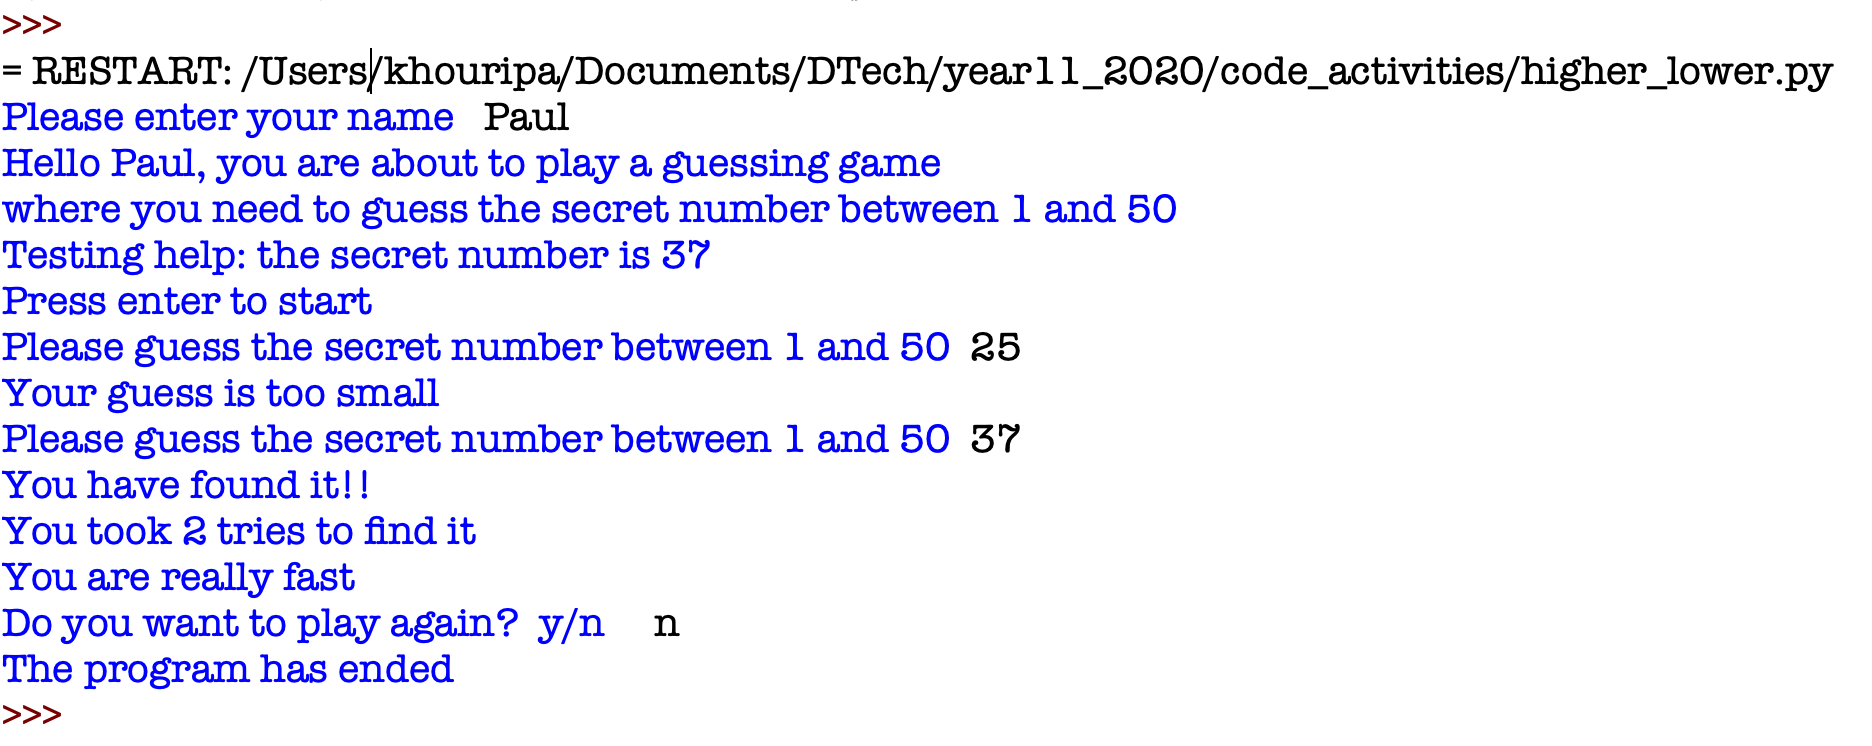
\includegraphics[width=17cm]{screen_shots/higher_lower.png}
\end{figure}
\newpage
\section{Validation}
When a user is making an input they may make an error and enter an \textbf{invalid} input.\\
This is an input that the program is not expecting:\\
Examples include:
\begin{itemize}
	\item Entering a string instead of a number (such as ``Two'' or ``Tracy'' when the program is expecting an integer or float).
	\item Entering nothing or a single letter , when the program wants a full name.
	\item Entering a letter ``outside of bounds'' (For example: the program expects one of A,B,C,D and the user enters F)
	\item Entering a number outside of bounds (For example, the program expects a number between 1 and 10 and the user enters 11).
	\item The program expects a single letter (``y'' or ``n''), but is given a word (``Yes'', ``No'').
	\item The program expects a capital letter (``A'') and is given a lower case letter (``a'').
\end{itemize}
Some of these entries can cause a program crash or just lead to poor ``performance'' of the program (for example: rejecting a user entry when what the user intended was valid).\\
The aim is always to make the program perform as well as possible and to be \textbf{User Friendly}.\\\\
To manage this \textbf{Usability} we need to \textbf{Validate} the user input.\\
This means one or both of two things:
\begin{itemize}
	\item If the user input is invalid, communicate the problem to the user and ask the user again for the entry
	\item Evaluate and possibly alter the user entry, so that its meaning is not changed but that it is formatted in a way that program expects. (An example of this is changing ``A'' to ``a''. \\ In this case the user does not need to be informed)
\end{itemize}


\newpage
\subsection{Integer Validation}
Consider an input request ``How many hamburgers would you like to order?''\\
\begin{itemize}
	\item We would expect this to be an integer with a value of 0 or more.
	\item Most likely we would like to ``operate'' on this later in the program (for example: multiply it by the cost of the hamburger to get a total price)
\end{itemize}
The input is always read as a string, so we need to cast the input to an integer.
\lstinputlisting[language=Python, caption=Python example]{validation_int_1.py}
This works properly \underline{assuming} the user enters a \underline{valid} input.\\
This is assumption is not good enough, and we need to deal with situations like the user entering $<$Enter$>$ or 3.5 or ``six''.\\
If they do, we get a program crash:
\begin{figure} [!h]
	\centering
	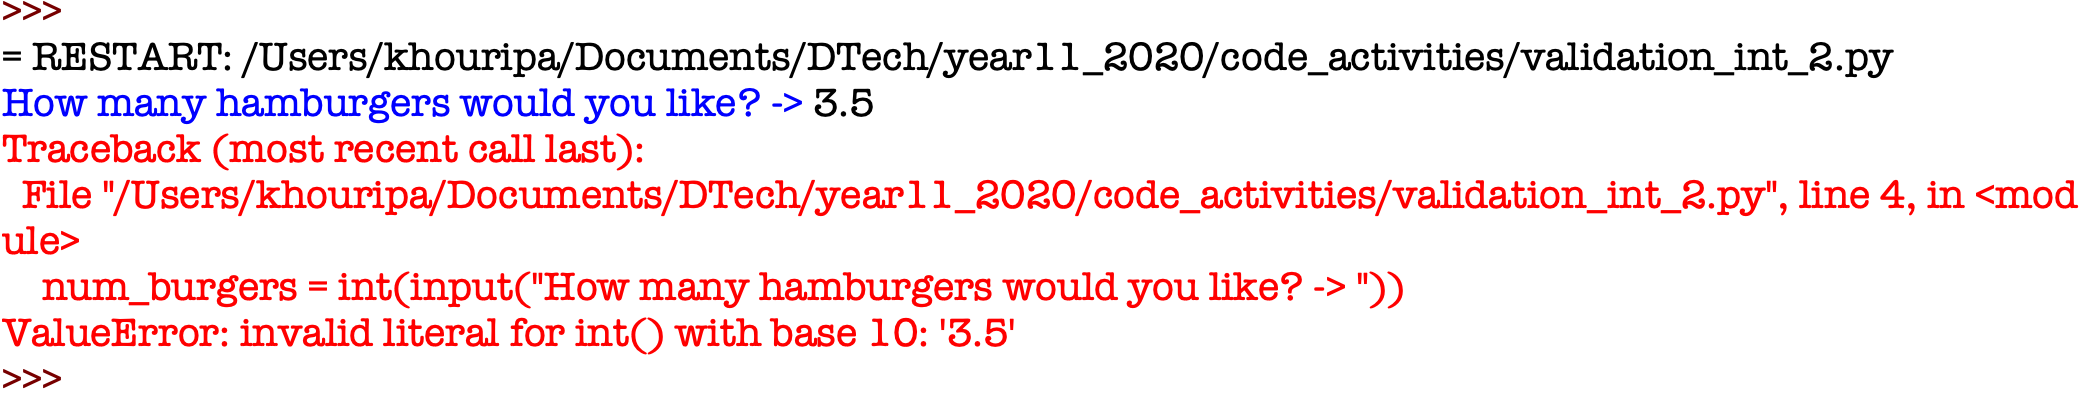
\includegraphics[width=17cm]{screen_shots/validation_int_1.png}
\end{figure}
To manage integer casting, we need a ``try except'' statement. This gets the program to do a check before accepting the cast.\\
The ``except ValueError'' will run if the input is not an integer.
\lstinputlisting[language=Python, caption=Python example]{validation_int_2.py}
\begin{figure} [!h]
	\centering
	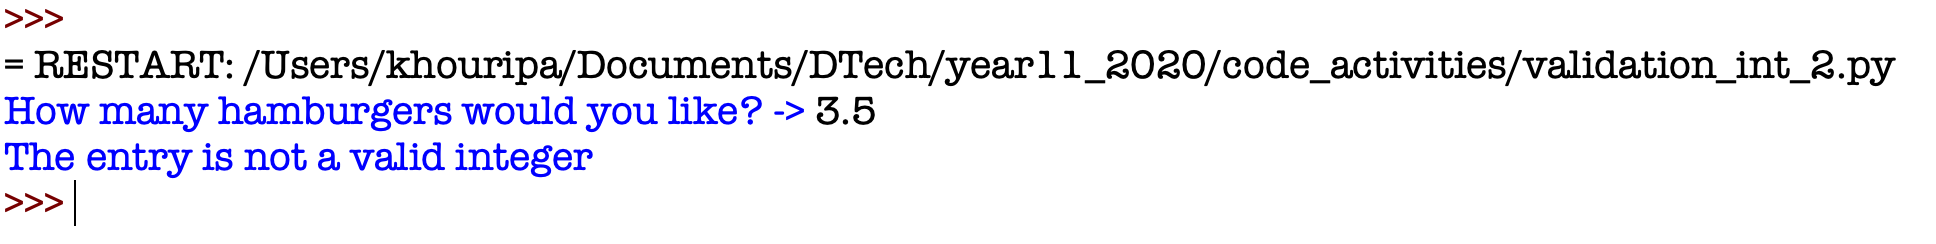
\includegraphics[width=17cm]{screen_shots/validation_int_2.png}
\end{figure}
This partly fixes the problem, but we still don't have an acceptable value for the number of hamburgers.\\
So we need to ask the user again for an input and if we want to ask again (and maybe again ....) we need a loop:

\lstinputlisting[language=Python, caption=Python example]{validation_int_3.py}
\begin{figure} [!h]
	\centering
	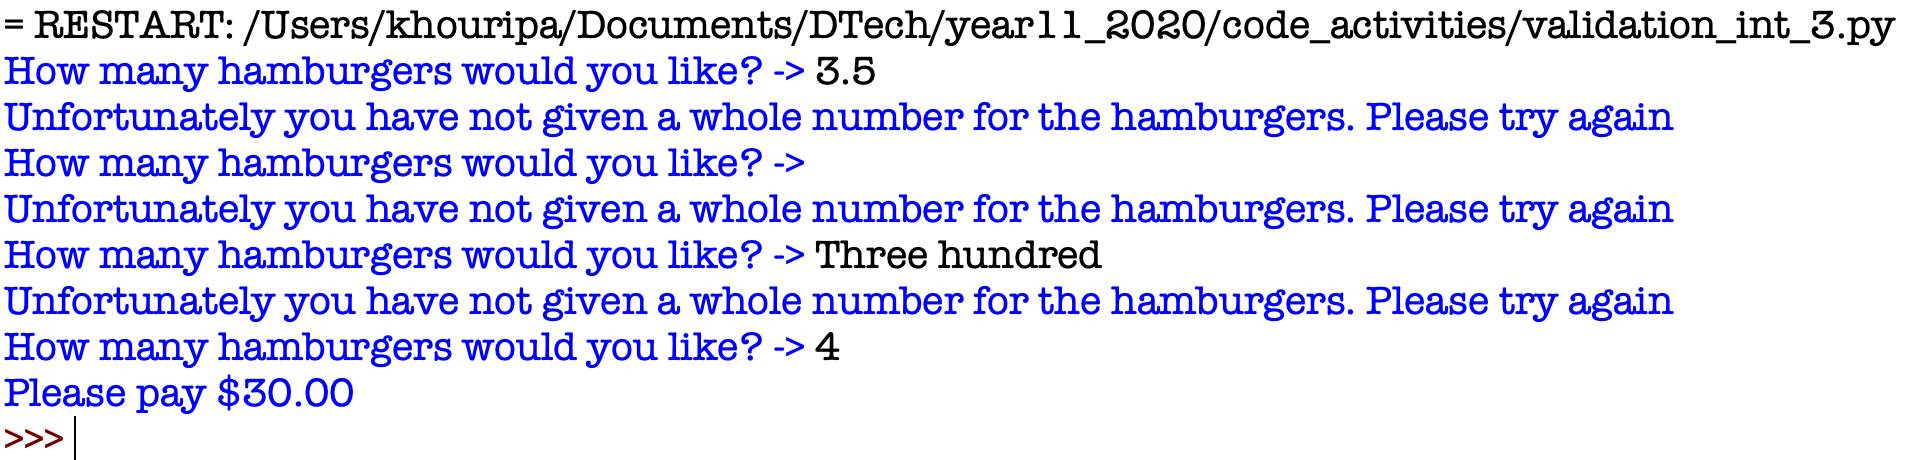
\includegraphics[width=17cm]{screen_shots/validation_int_3.png}
\end{figure}
 We still have a problem that the program accepts negative numbers:
 
 \begin{figure} [!h]
 	\centering
 	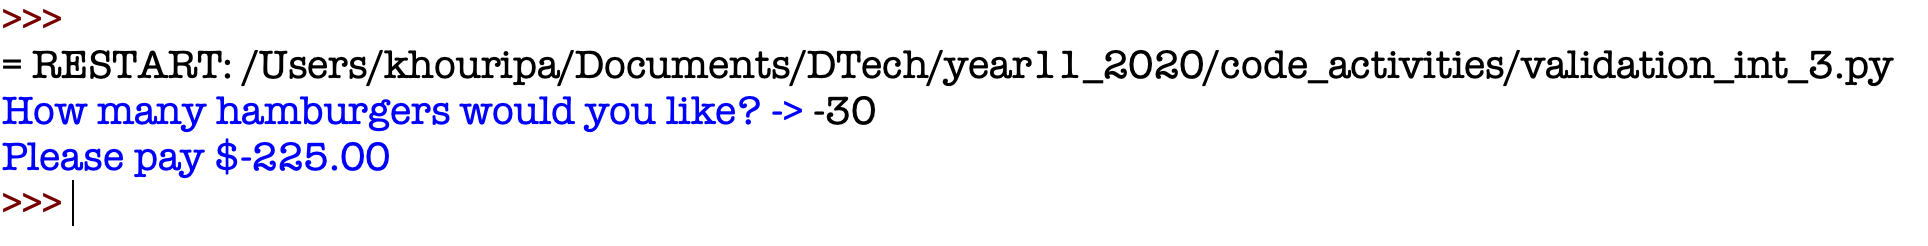
\includegraphics[width=17cm]{screen_shots/validation_int_3_neg.png}
 \end{figure}

So we can extend the the validation loop
\lstinputlisting[language=Python, caption=Python example]{validation_int_4.py}
 \begin{figure} [!h]
	\centering
	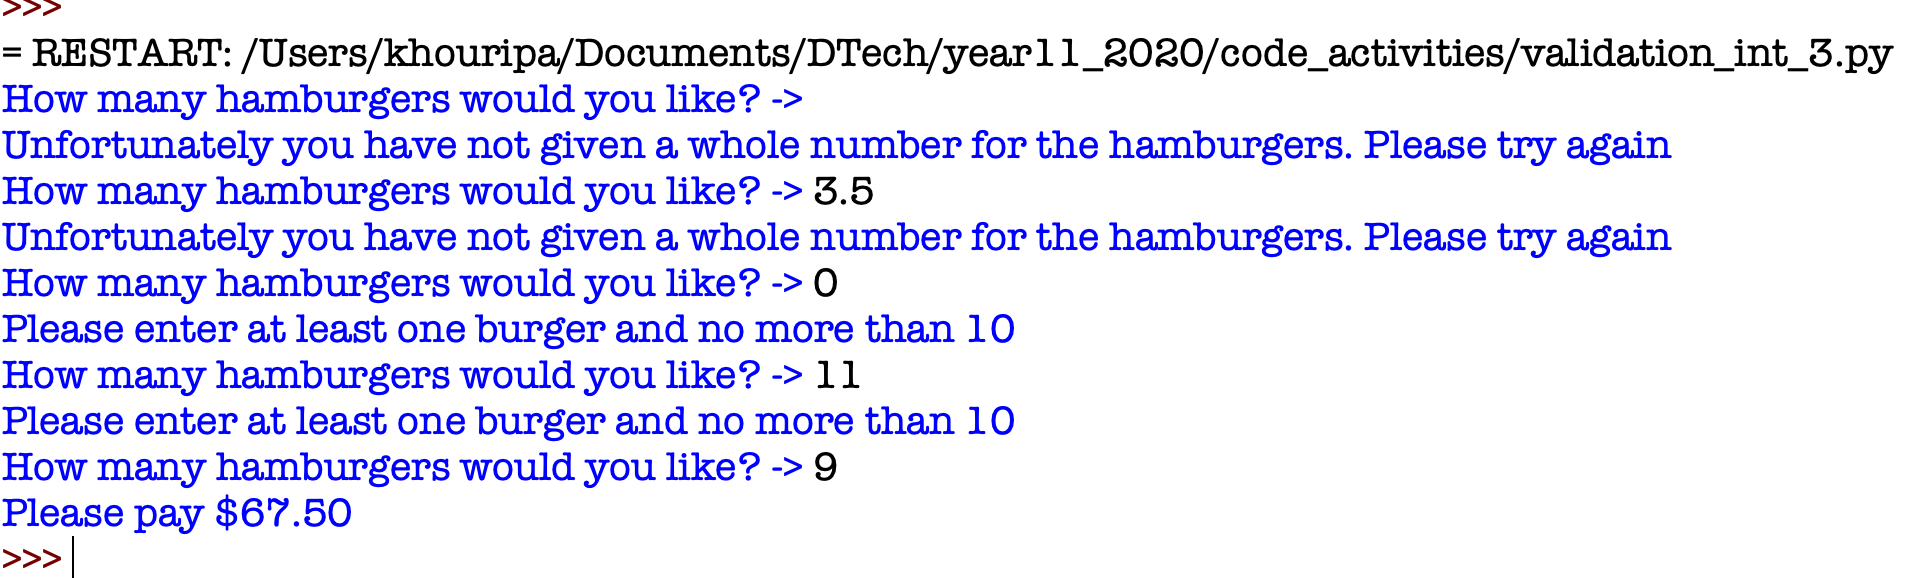
\includegraphics[width=17cm]{screen_shots/validation_int_4.png}
\end{figure}
\newpage
 \subsection{String Validation}
 If we require a name, we still need to check that we are getting something acceptable.\\
 A simple validation can be to check that the entry has at least 2  characters and no more than (maybe) 20 (what do you think is the longest number of characters that can be in a name?).
 
 \lstinputlisting[language=Python, caption=Python example]{validation_name.py}
 \begin{figure} [!h]
 	\centering
 	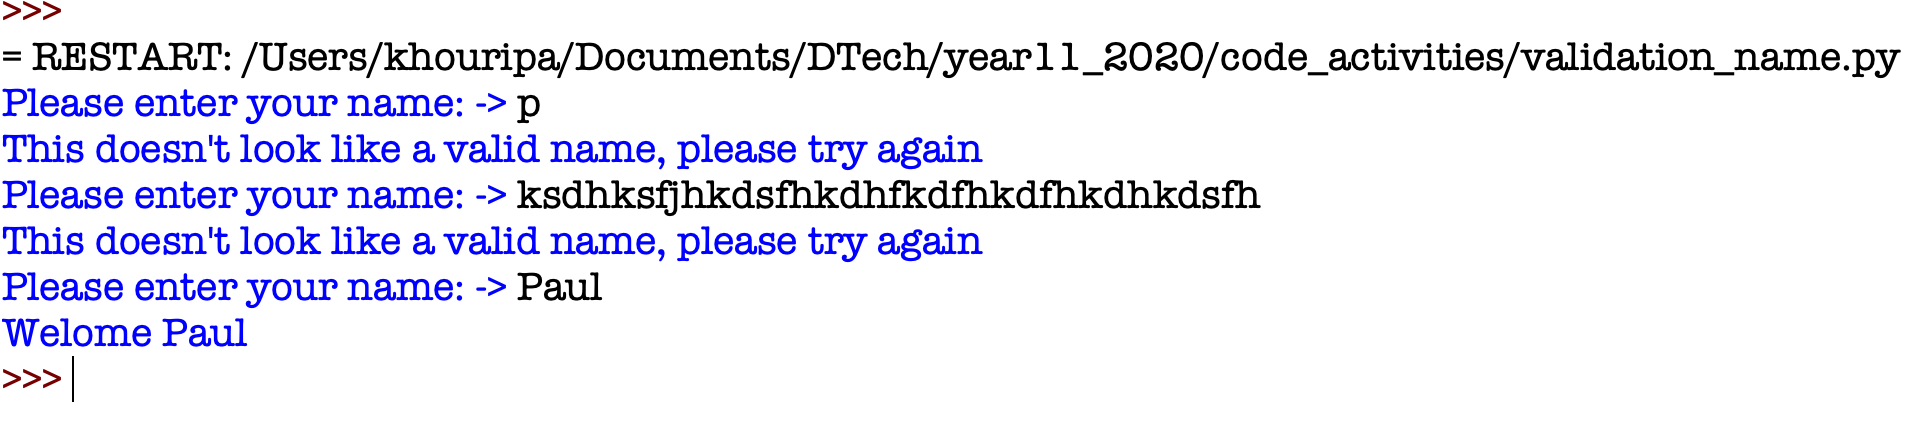
\includegraphics[width=17cm]{screen_shots/validation_name.png}
 \end{figure}

This validation checks that the characters in the name are all acceptable (i.e no numbers or special characters).\\
It does this by checking each character in the name against a list of characters than are acceptable.

 \lstinputlisting[language=Python, caption=Python example]{validation_name_1.py}
\begin{figure} [!h]
	\centering
	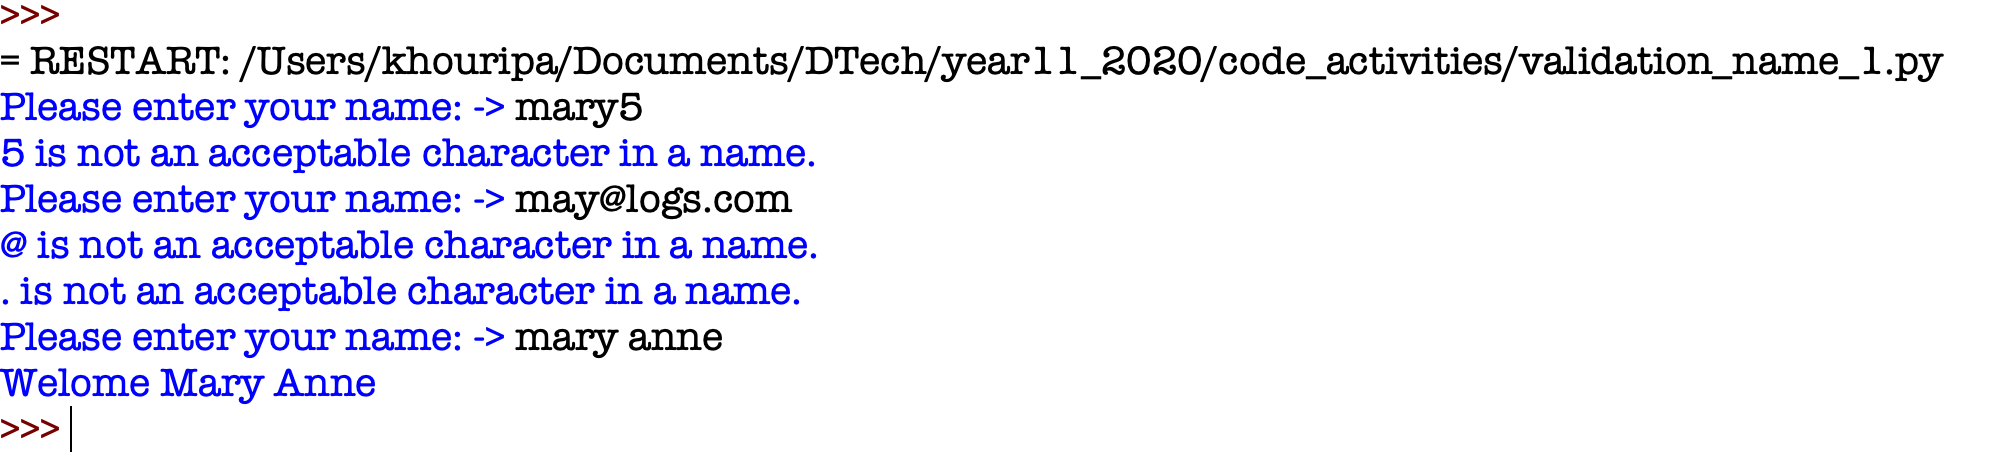
\includegraphics[width=17cm]{screen_shots/validation_name_1.png}
\end{figure}
 
 \begin{itemize}
 	\item Checking that strings follow an acceptable ``pattern'' is called ''regular expressions'' and this is outside of the scope of Level 1 (but we can explore options like in the code example).\\
 	\url{https://www.w3schools.com/python/python_regex.asp}
 	\item It is also a good idea to be familiar with ``string methods'' as they can be very useful.\\
 	\url{https://www.w3schools.com/python/python_strings_methods.asp}
 \end{itemize}




\newpage
\section{Lists}
Quite often we want to store a whole set of items (for example, names). Having a variable for each one is not very helpful (particularly if we want to add more names to the lists or remove some names).\\
Suppose we have a small class of 6 students and we want to store all of their names.\\
There names are: Agatha , Melinda, Harriet, Hine, Dandelion and Te Aroha\\
To create a list we use square brackets and commas.
\lstinputlisting[language=Python, caption=Python example]{list_base.py}
To manage lists, there are a large range of methods that can be used.\\
See the examples below.
\lstinputlisting[language=Python, caption=Python example]{list_base_1.py}
See also:
\begin{itemize}
	\item Python Lists:  \url{https://www.w3schools.com/python/python_lists.asp}
	\item Python List Methods: \url{https://www.w3schools.com/python/python_lists_methods.asp}
\end{itemize}



\section{Lists and Loops}
\subsection{Creating and modifying a class group}
\textbf{Scenario:}\\
Create a simple program that asks the user to enter the names for students in a class.\\
Once the names have been entered it prints out the names as a numbered list.\\
Extension:\\
One the names have been entered and listed, ask the user if they would like to modify or remove any of the names.
(and if they do allow them to do it)







\subsection{Lucky Unicorn Game}
\subsubsection{Program}
\textbf{Scenario:}\\
You have decided to create a fun game to raise money for the charity Doctors without Borders.\\ 
You will set up your computer at lunchtime and players will pay to play.  \\

\textbf{Here are the rules:}\\
Users pay an initial amount at the start of the game. 
\begin{itemize}
	\item The cost should be \$1 per round and users should press $<$enter$>$ to play.  
	\item The computer should then generate a token that is either a zebra, horse, donkey or unicorn.  
	\item This should be displayed to the user (as text). 
	\item If the token is a unicorn, the user wins \$5, if it is a zebra or horse, they win 50c and if it is a donkey then they don’t win anything. 
\end{itemize}
\hrule \vspace{0.5cm}

The maximum amount of money that students can spend on the game is \$10 per session. 
 \begin{itemize}
	\item The game should allow players continue / quit provided they have not lost all of their money. 
	\item  It should supply appropriate feedback so that the user knows how much money they have won / lost each round and how much money they have left.
\end{itemize}
\hrule \vspace{0.5cm}

Once students have no more money, the game should end (although players do have the option of quitting while they are ahead).\\

\hrule \vspace{0.5cm}


Variations (optional)
Once you have a working game, you are welcome to develop the outcome further.  \\
Here are some variations you could consider…
\begin{itemize}
	\item Change the tokens / context ( so rather than having zebra, horses, donkeys and unicorns the game could involve other items )
	\item Allow users to bet more than \$1 per round and adjust the pay-outs proportionally\\ 
(be careful to set up you game so that the house has a long term advantage)
\end{itemize}


\newpage
\subsubsection{Planning: Iterative Processes}
\begin{itemize}
	\item Break the problem down into parts (Draw some kind of diagram)
	\item Each of the parts can be called a ``component'' of the program or a ``sub-problem''.
	\item You need plan and test code for each of these ``sub-problems''.
	\begin{itemize}
		\item Ideally (and this must happen somewhere), you need to look at ``trialling'' different ways to solve the sub-problem), with the idea being that you can trial the different ways and choose the best (and also look to ways of improving). \\
		This needs to be captured in the planning documentation for the iterative processes assessment.
	\end{itemize}
	\item Combine your code into a fully working program (your first version)
	\begin{itemize}
		\item Test the program and document the test (gridded test plan)
		\item Write a short reflection on what works and what could be improved upon.
	\end{itemize}
\item Plan the next version 
\begin{itemize}
	\item Test the program and document the test (gridded test plan)
	\item Write a short reflection on what works and what could be improved upon.
\end{itemize}
\item Repeat this planning and testing process.
\item If new sub-problems appear , then work on them in the same way as referred to above
\end{itemize}
\newpage

\begin{figure} [!h]
	\centering
	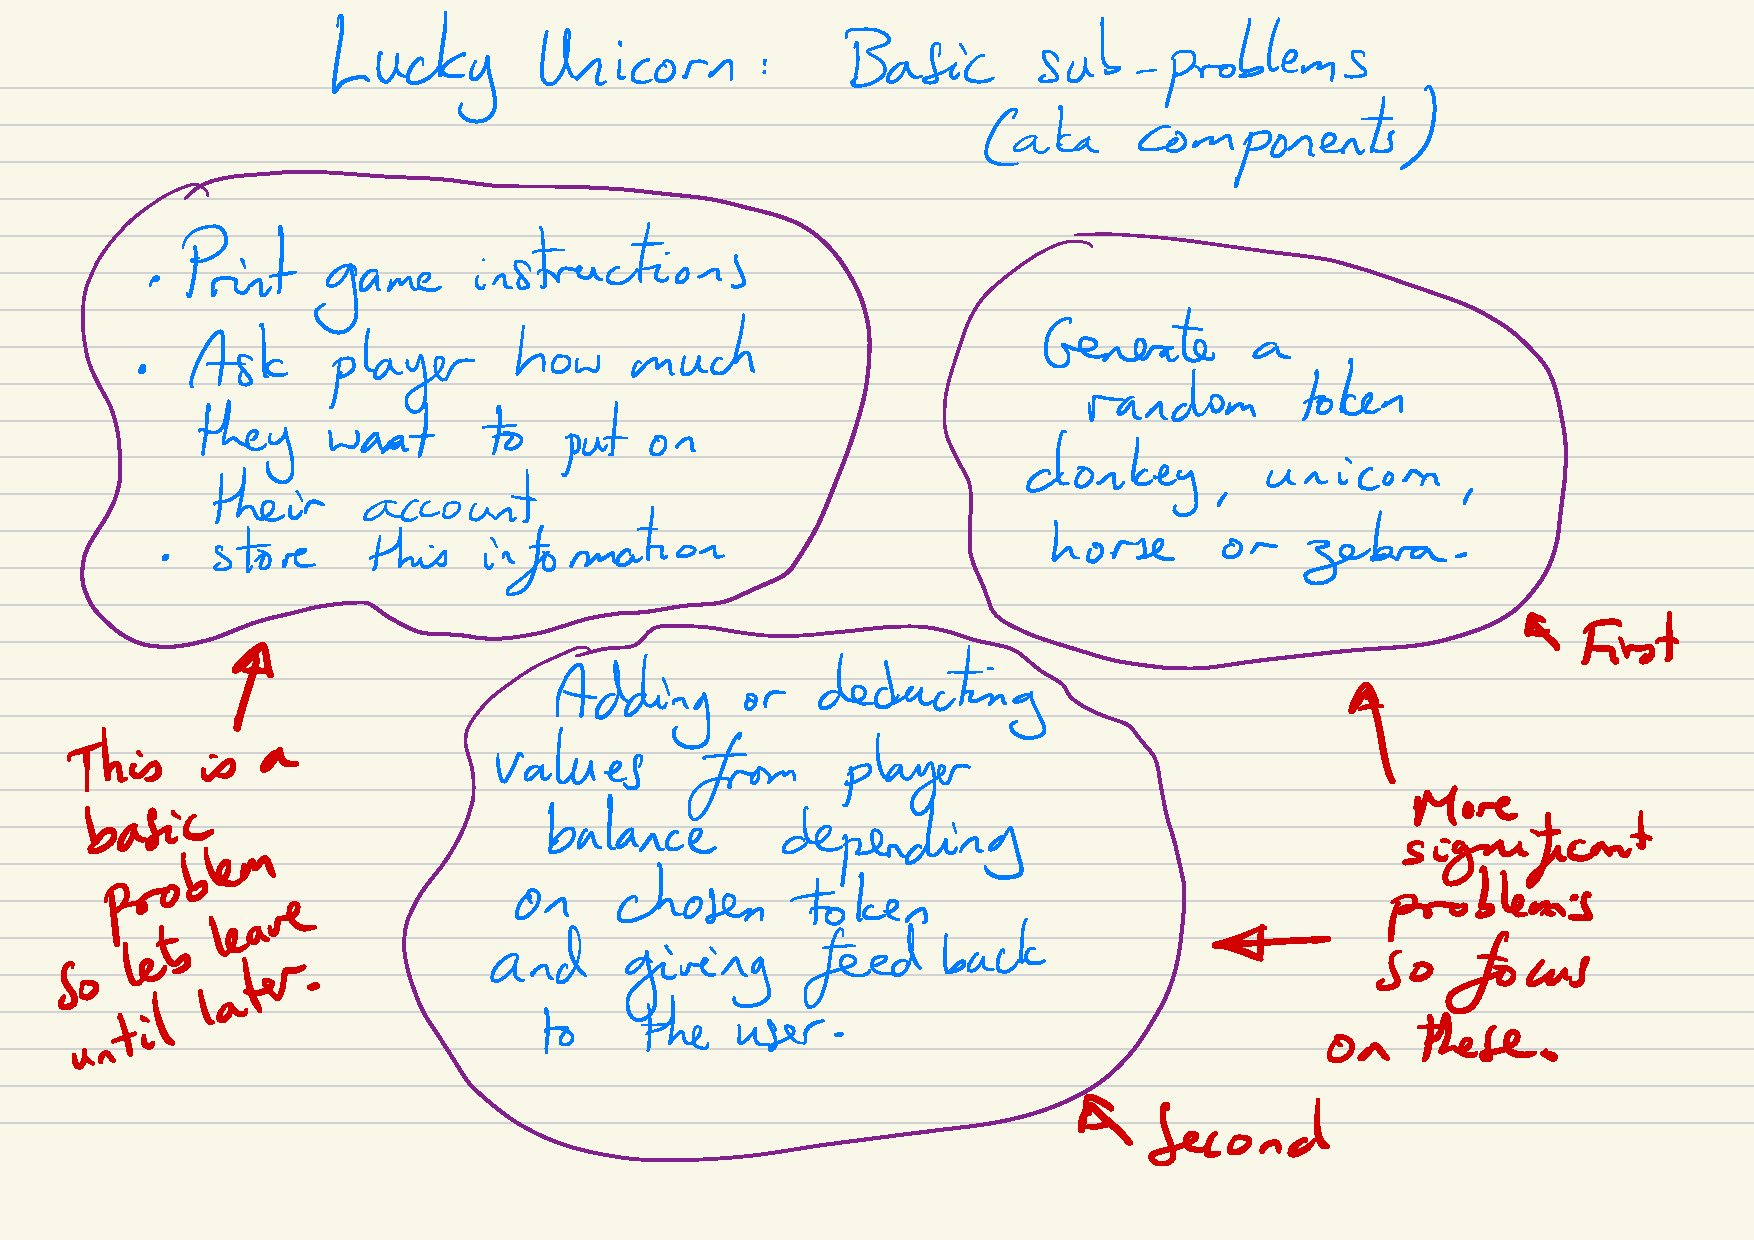
\includegraphics[width=15cm]{iterative_processes/Lucky_Unicorn_Sub_problems_1.pdf}
	\caption*{Breaking the problem down into components}
\end{figure}

\begin{figure} [!h]
	\centering
	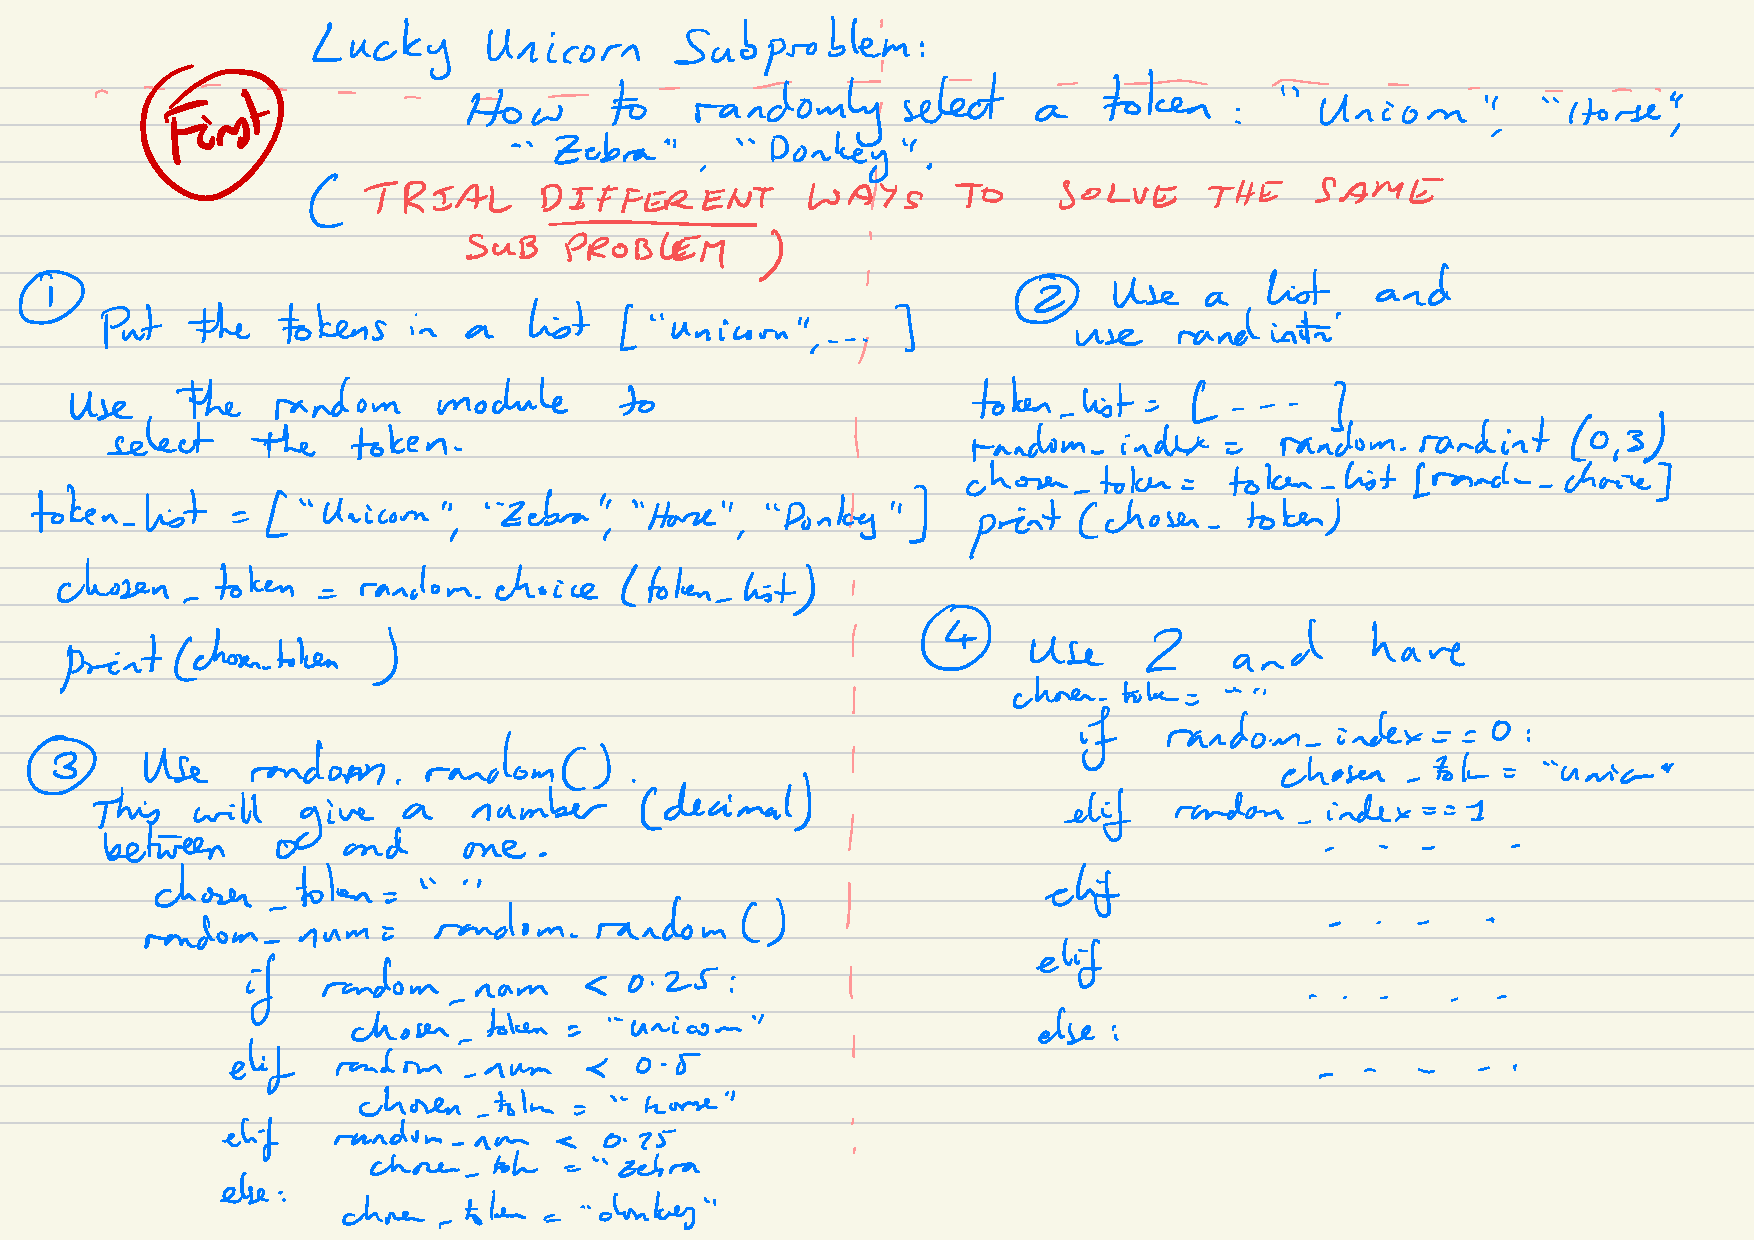
\includegraphics[width=15cm]{iterative_processes/Lucky_Unicorn_Sub_problems_2.pdf}
	\caption*{Planning options for the first sub-problem}
\end{figure}

\newpage

\begin{figure} [!h]
	\centering
	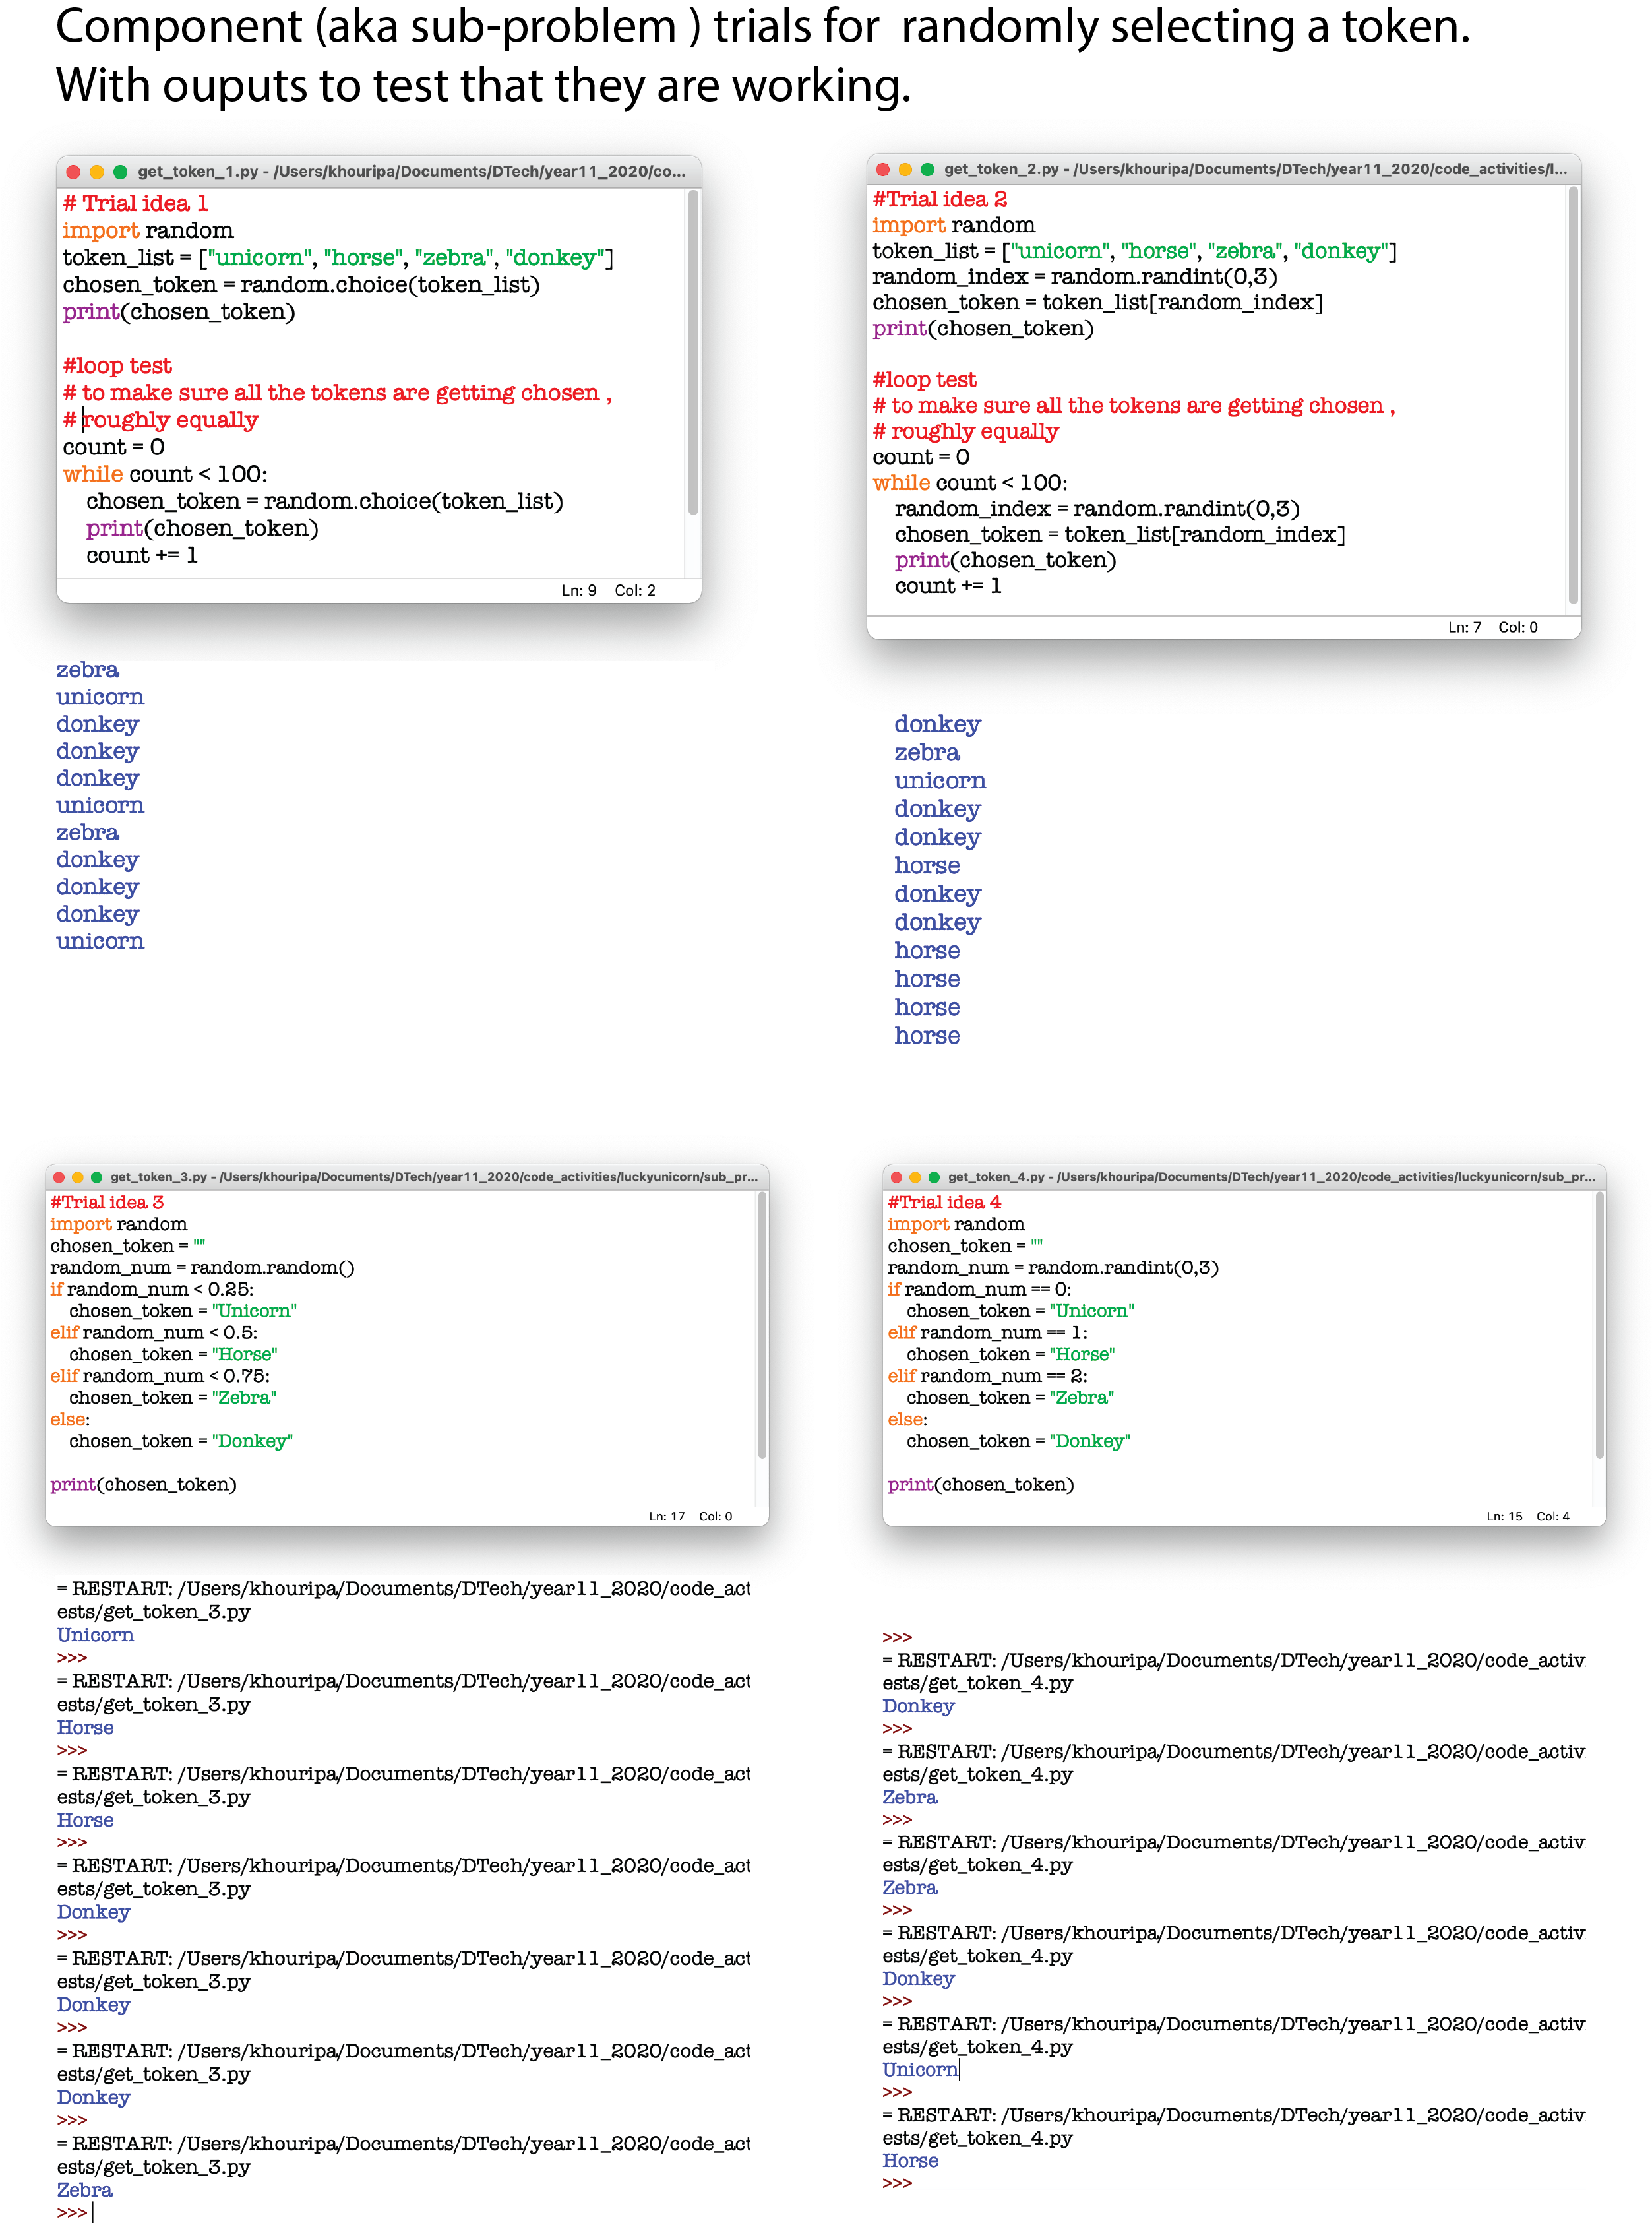
\includegraphics[width=17cm]{iterative_processes/sub_problem_trials.png}
	\caption*{Trialling different ways to solve the same sub-problem}
\end{figure}

\newpage

\begin{figure} [!h]
	\centering
	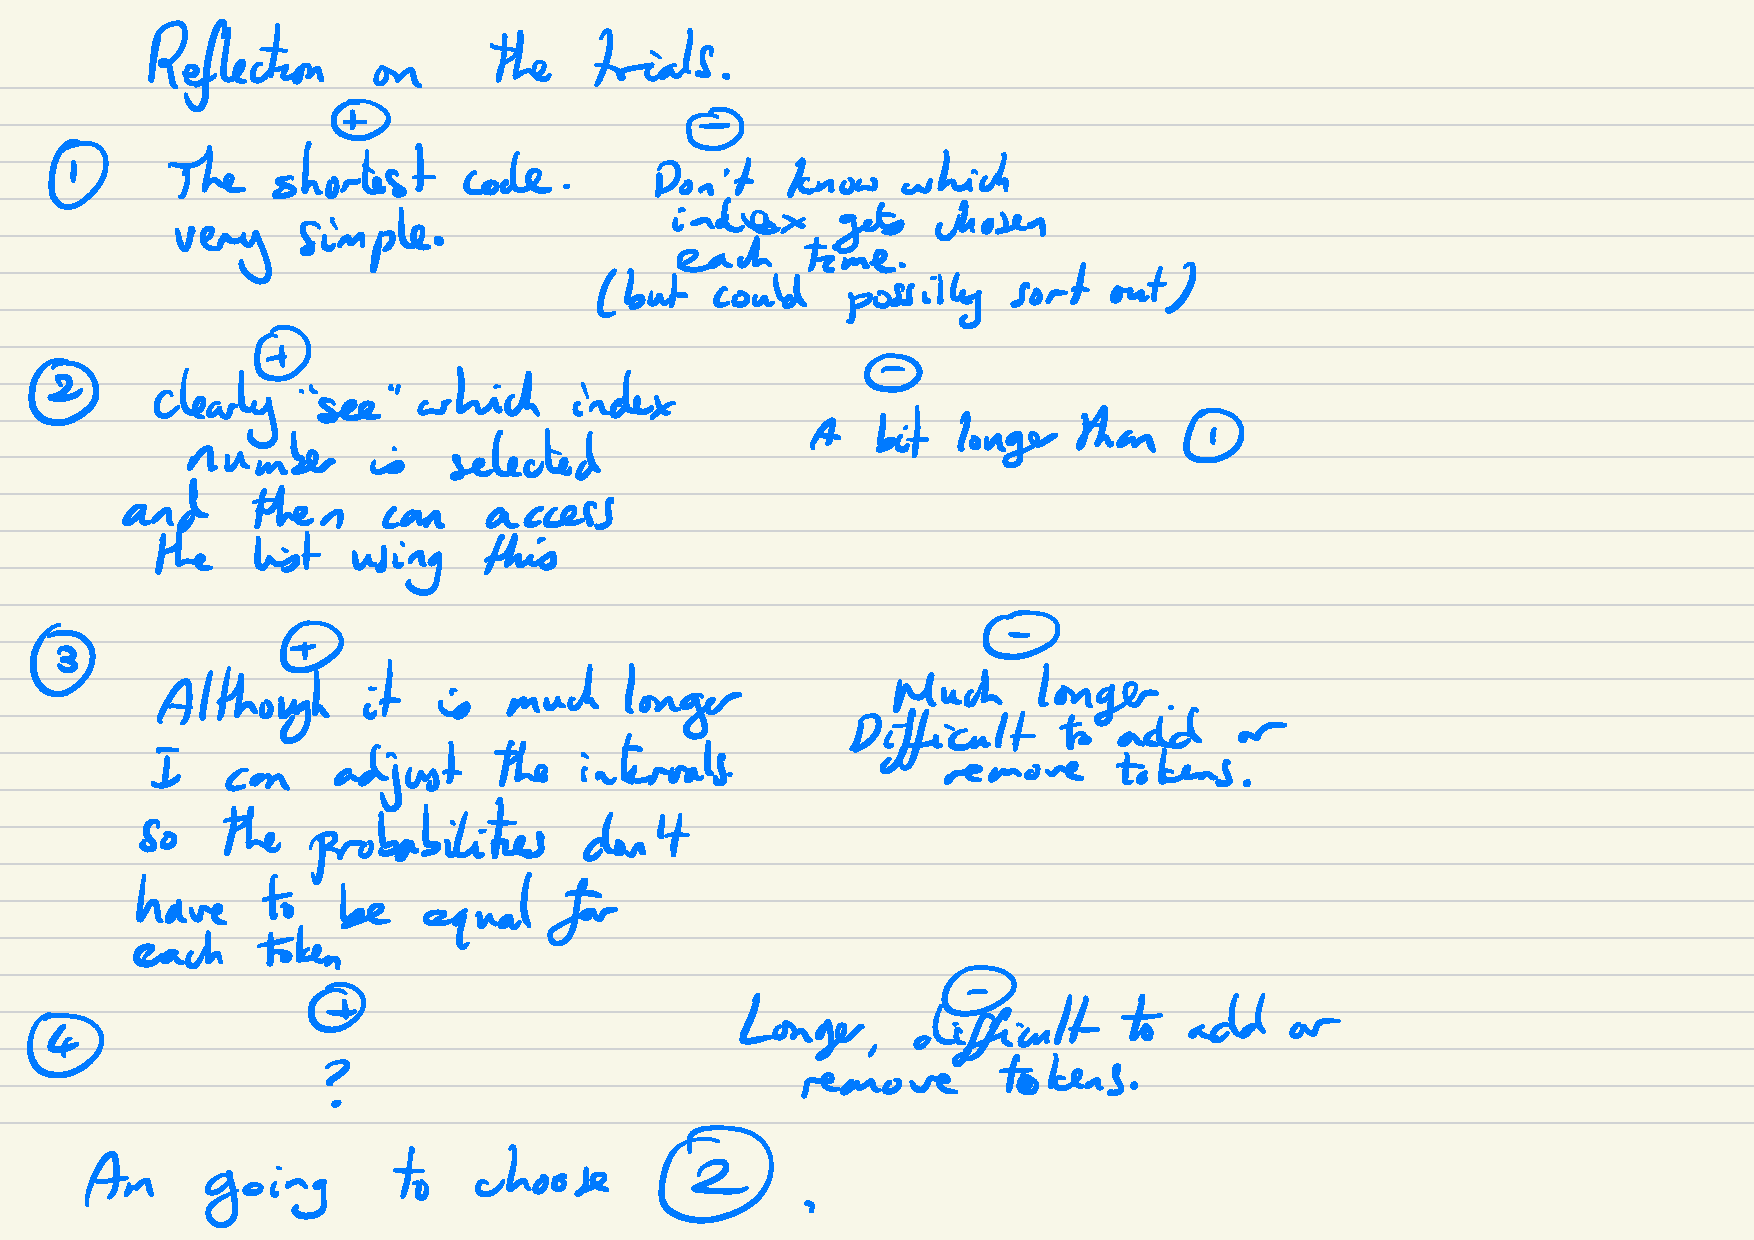
\includegraphics[width=15cm]{iterative_processes/Lucky_Unicorn_Sub_problems_2_a.pdf}
	\caption*{A reflection on the trials and a choice}
\end{figure}

\begin{figure} [!h]
	\centering
	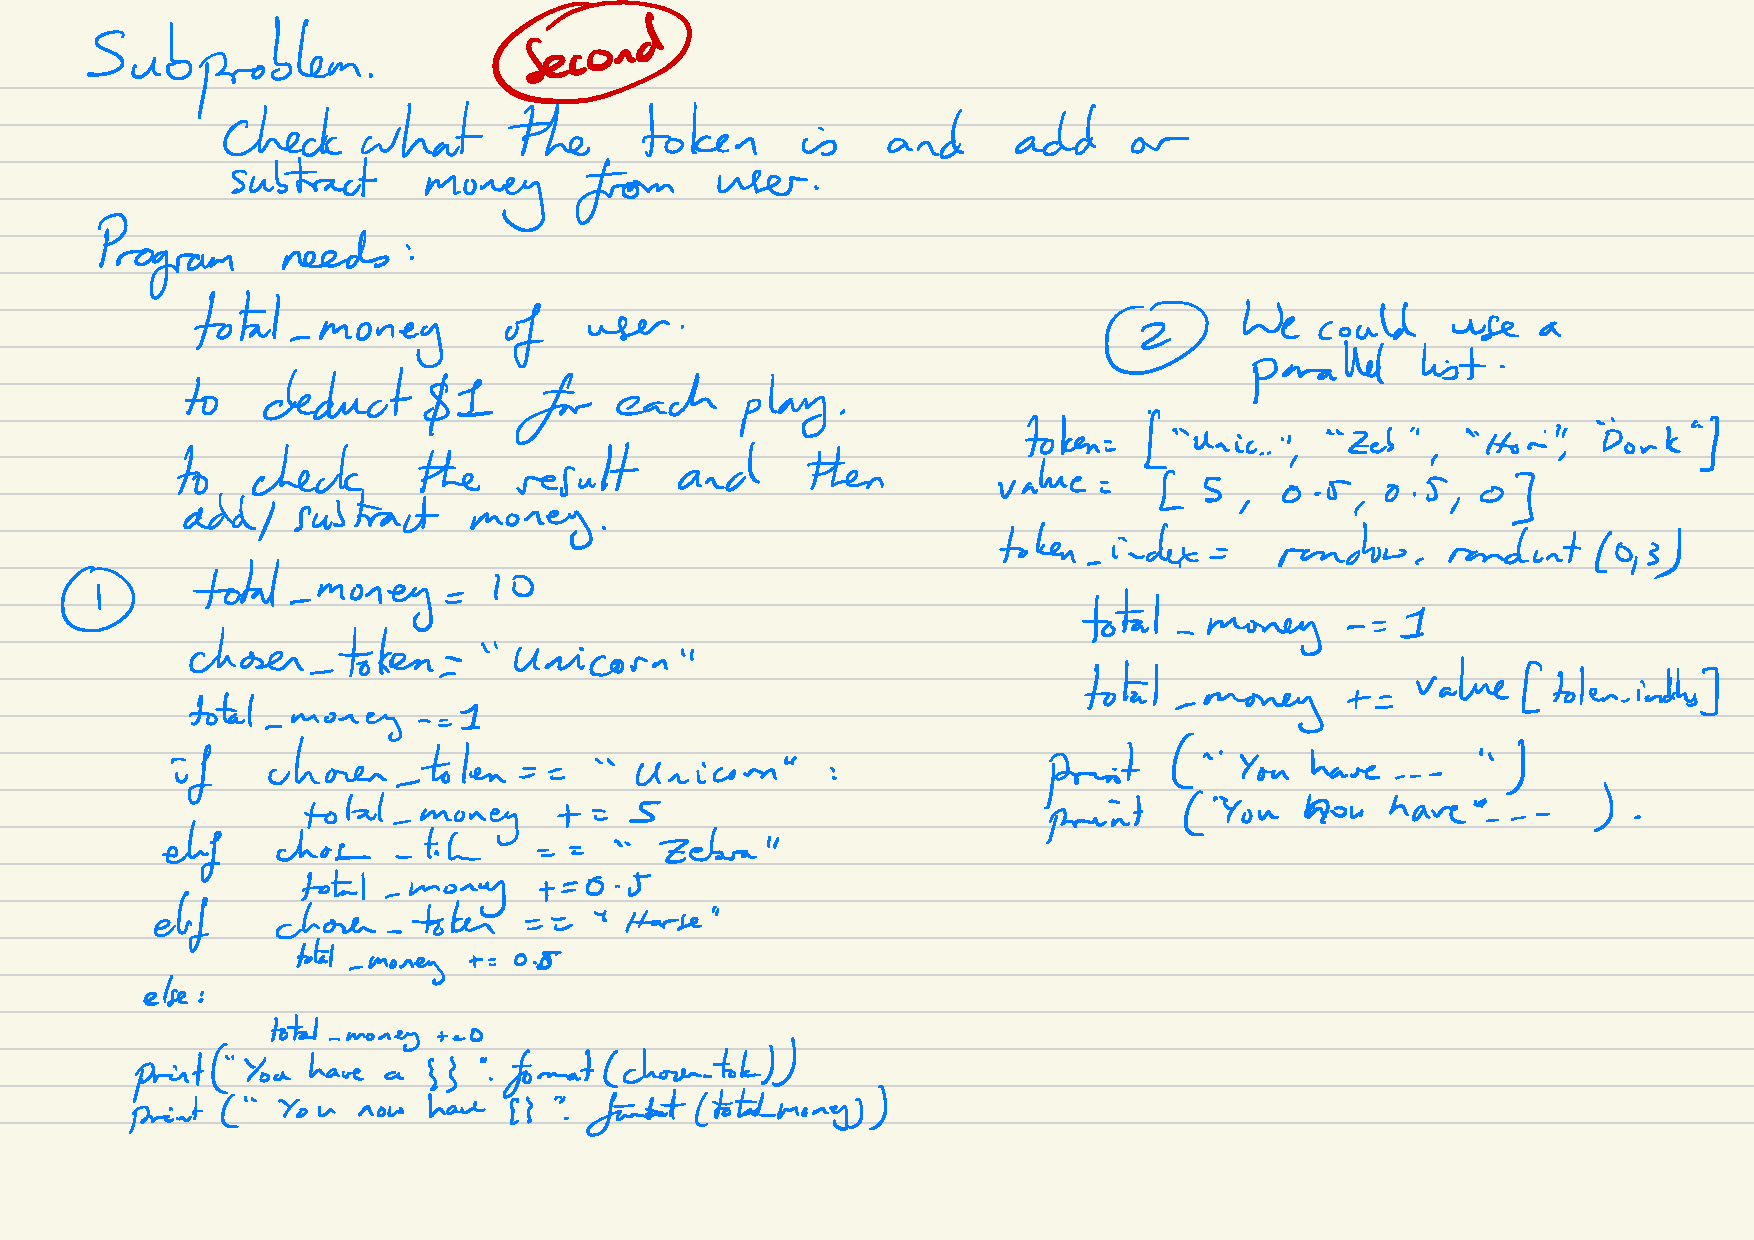
\includegraphics[width=15cm]{iterative_processes/Lucky_Unicorn_Sub_problems_3.pdf}
	\caption*{Planning options for the second sub-problem}
\end{figure}
\newpage

\begin{figure} [!h]
	\centering
	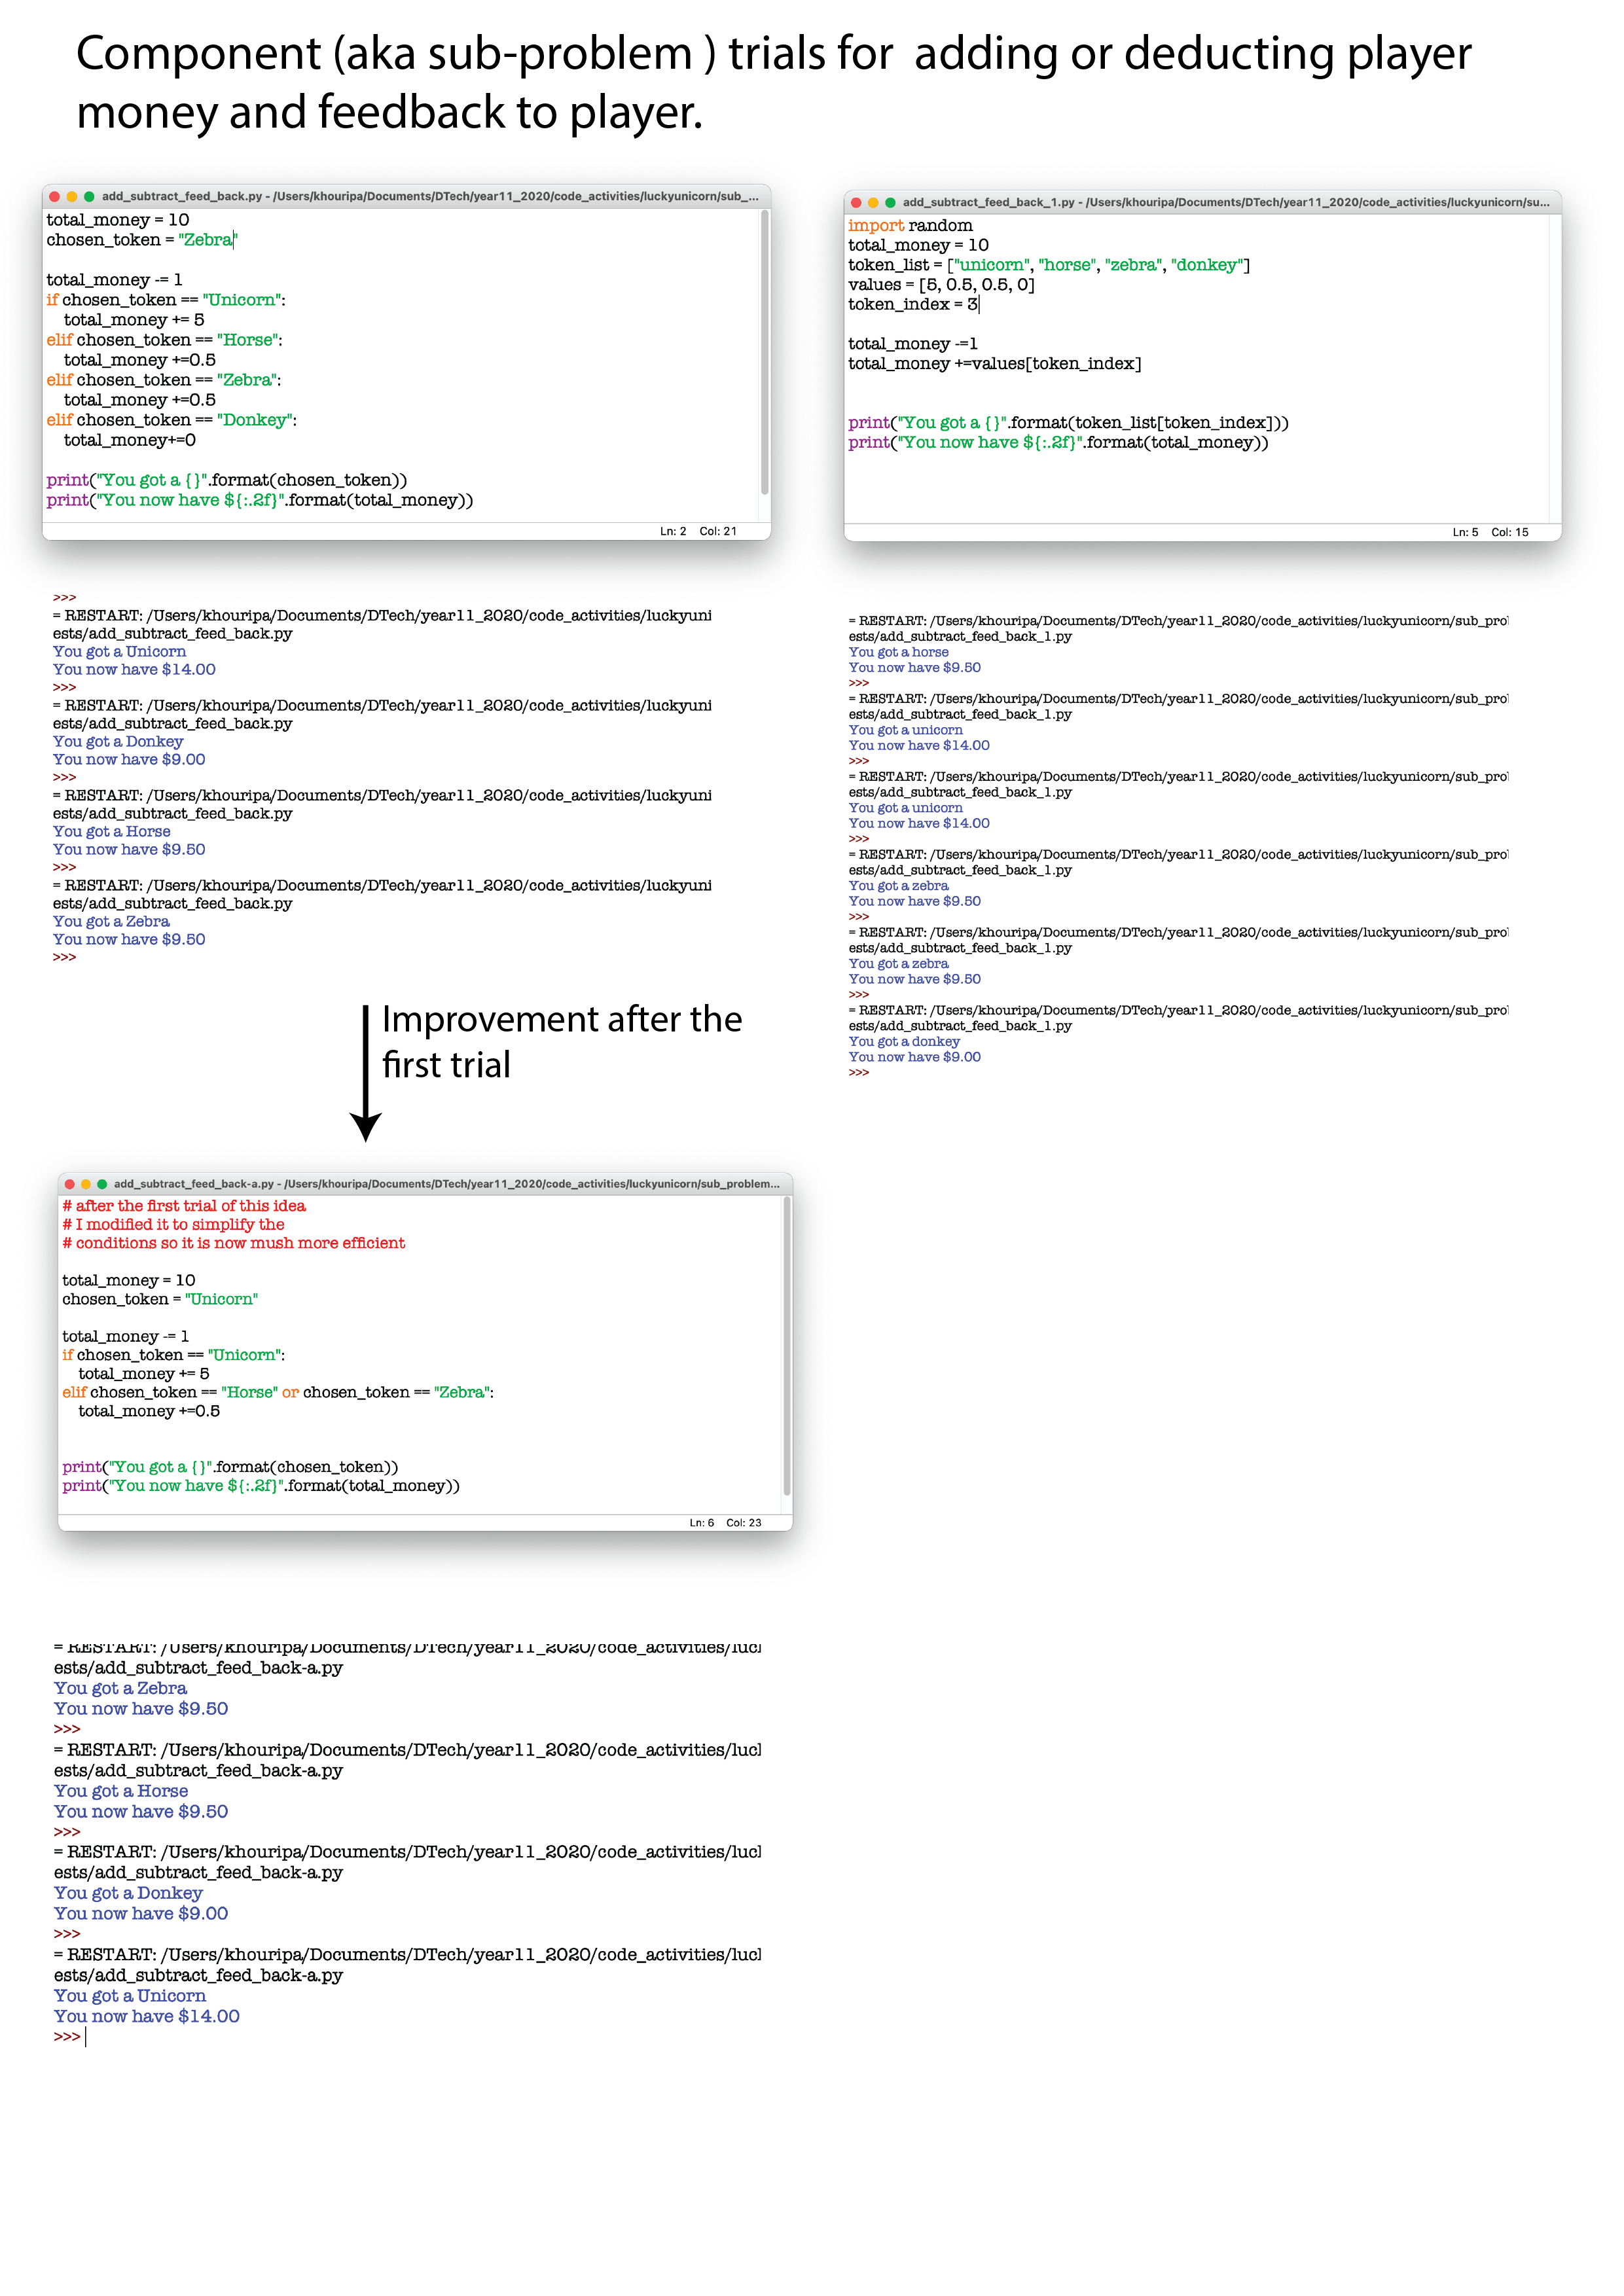
\includegraphics[width=17cm]{iterative_processes/sub_problem_trials_2.png}
	\caption*{Trialling different ways to solve the same sub-problem (the second)}
\end{figure}

\newpage

\begin{figure} [!h]
	\centering
	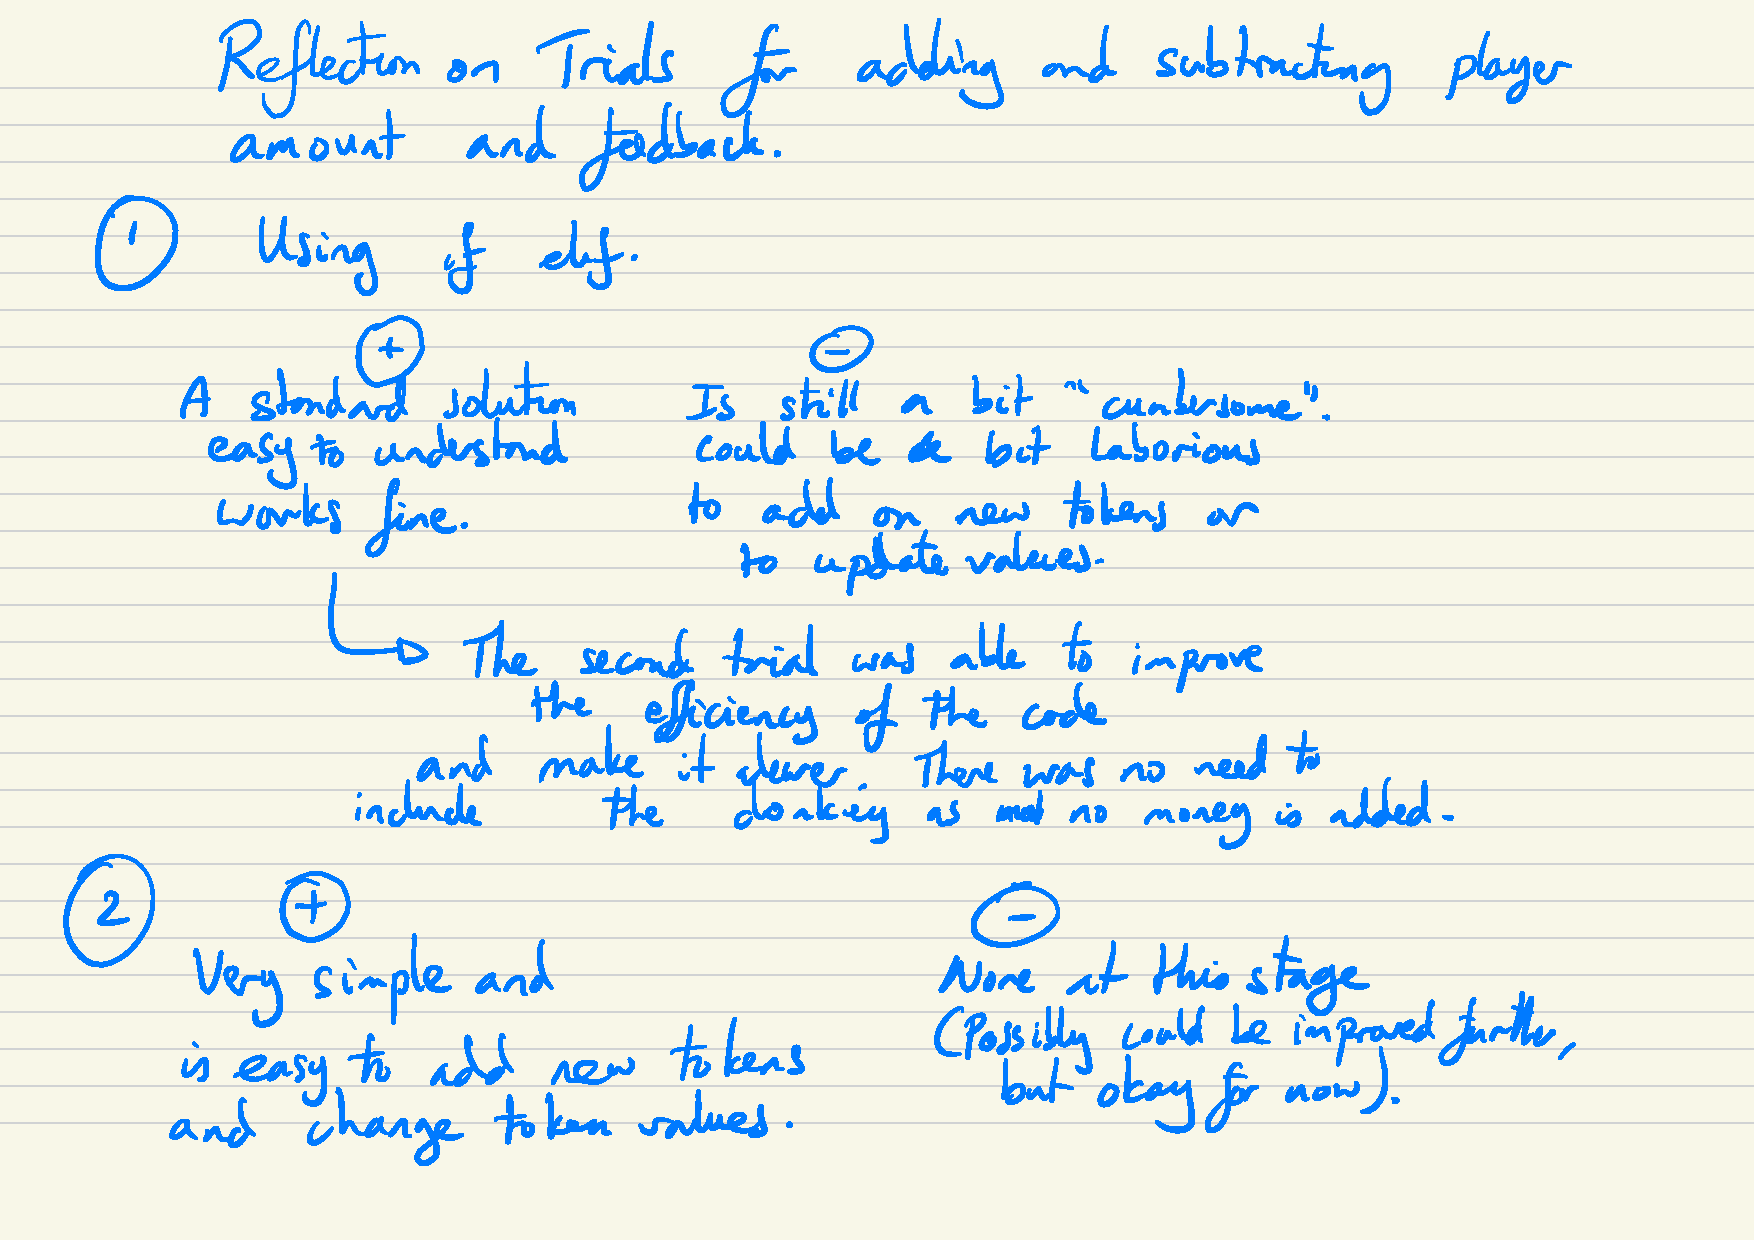
\includegraphics[width=15cm]{iterative_processes/Lucky_Unicorn_Sub_problems_3_a.pdf}
	\caption*{A reflection on the trials and a choice}
\end{figure}

\newpage
\lstinputlisting[language=Python, caption=Python example]{luckyunicorn/v1_lucky_unicorn.py}
\newpage

\section{Functions}
\lstinputlisting[language=Python, caption=Python example]{addition_question.py}
\lstinputlisting[language=Python, caption=Python example]{function_tests.py}
\newpage
\section{Testing}
\newpage
\section{Dictionaries}
\lstinputlisting[language=Python, caption=Python example]{dictionaries.py}
\lstinputlisting[language=Python, caption=Python example]{tommi.py}



\newpage
\section{Coffee}
\lstinputlisting[language=Python, caption=Python example]{class_randomletters_function.py}
\lstinputlisting[language=Python, caption=Python example]{buildingastring.py}
\lstinputlisting[language=Python, caption=Python example]{buildingastring_v2.py}
\lstinputlisting[language=Python, caption=Python example]{buildingastring_v3.py}
\lstinputlisting[language=Python, caption=Python example]{class_randomletters_testfor6.py}
\lstinputlisting[language=Python, caption=Python example]{class_randomletters_function_c_list.py}
\lstinputlisting[language=Python, caption=Python example]{class_randomletters_function_list.py}
\lstinputlisting[language=Python, caption=Python example]{class_randomletters_testfor7.py}
\lstinputlisting[language=Python, caption=Python example]{class_randomletters_testfor8.py}
\lstinputlisting[language=Python, caption=Python example]{class_randomletters.py}
\lstinputlisting[language=Python, caption=Python example]{class_randomletters_function_c.py}
\lstinputlisting[language=Python, caption=Python example]{class_randomletters_to_distribution.py}
\newpage
\section{Tests}
\lstinputlisting[language=Python, caption=Dice Roll]{v0_random.py}
\lstinputlisting[language=Python, caption=Python example]{checkinlist.py}
\lstinputlisting[language=Python, caption=Python example]{dictionary_test.py}
\lstinputlisting[language=Python, caption=Python example]{format_test.py}
\lstinputlisting[language=Python, caption=Python example]{hangman.py}
\section{Strings}
\lstinputlisting[language=Python, caption=Python example]{string_tests.py}
\lstinputlisting[language=Python, caption=Python example]{counting_string.py}
\section{Objects}
\lstinputlisting[language=Python, caption=Python example
]{classes_objects.py}

\lstinputlisting[language=Python, caption=Python example
]{classforglobals.py}

\lstinputlisting[language=Python, caption=Python example
]{class_quiz.py}













\end{document}